% ----------------------------------------------------------------------------------------------------- %
% Manual da Classe UFTeX
% 
% Versão 2.1:   Março 2018
%
% Criado por:   Tiago da Silva Almeida
% Revisado por: Tiago da Silva Almeida
%               Rafael Lima de Carvalho
%               Ary Henrique Morais de Oliveira
%
% https://almeidatiago.github.io/uftex/
% ----------------------------------------------------------------------------------------------------- %

\documentclass[tcc1]{uftex}
% ---- Esse comando cria o nome uftex estilizado
\newcommand\uftex{UF\TeX}
\usepackage[font=small,labelfont=bf]{caption}
\usepackage{lipsum}
\usepackage{tikz}
\usepackage{indentfirst}
\usepackage[siunitx]{circuitikz}
\usetikzlibrary{arrows}
\usepackage[alf,abnt-emphasize=bf]{abntex2cite}
\renewcommand{\backrefpagesname}{}
\renewcommand{\backref}{}
\renewcommand*{\backrefalt}[4]{}
\setlength{\parindent}{1.25cm}
% ----  Esse comandos são necessário no pré-ambulo para a impressão da lista de lista abreviatuas e de símbolos
\makelosymbols


\makeloabbreviations 


% ---- Início do documento 


\begin{document}
  % ---- Descrição do título do trabalho 
  \title{Análise de dados para encontrar características e sintomas em comum entre os pacientes de covid-19 no brasil}
  % ---- Nome do autor ou autores do trabalho
  \author{Renato}{Luiz de Almeida}
  % ---- Nome do orientador do trabalho. O último campo representa o título do professor
  \advisor{Prof.}{George}{Lauro Ribeiro de Brito}

  \examiner{Prof.}{Dr.}{Nome do Primeiro Examinador Sobrenome}
  \examiner{Profa.}{Dra.}{Nome do Segundo Examinador Sobrenome}
  \examiner{Profa.}{Ma.}{Nome do Terceiro Examinador Sobrenome}
  % ---- Departamento representa o curso ao qual o trabalho está sendo apresentado. Descrito por meio de duas iniciais do curso
  \department{CC}
  % ---- Data da apresentação do trabalho
  \date{22}{12}{2021}
  % ---- Palavras-chaves em português do trabalho
  \keyword{Mineração de Dados}
  \keyword{Covid-19}
  \keyword{KDD}
  \keyword{Pandemia}
  % ---- Comando responsável por criar a capa do trabalho e/ou folha de resto conforme a configuração exigida
  \maketitle

  \frontmatter

  % ----------------------------------------------------------------------------------------------------- %
  %  Este trecho deve ser inserido somente no caso do TCC2 já na versão FINAL
  % ----------------------------------------------------------------------------------------------------- %
  
\includepdf{ficha_catalografica}
  
\includepdf{ata_de_aprovacao}
  % ----------------------------------------------------------------------------------------------------- %
  \dedication{A algu\'em cujo valor \'e digno desta dedicat\'oria.}

  \begin{acknowledgement}
  Gostaria de agradecer a todos.
  \end{acknowledgement}

  \begin{abstract}
  \setlength{\parindent}{1.25cm}
    No final de 2019 surgia uma perigosa variante do vírus da covid, a SARS-CoV-2, esse que causa a covid-19. Esse novo vírus provocou uma pandemia mundial que se estende até os dias de hoje, ele se espalhou rapidamente por todo o globo provocando a contaminação de grande parte da população. Essa pandemia nos colocou diante de grande numero de doentes e mortos, por esse auto nível de gravidade, surgiu danos profundos em nossa sociedade, sendo alguns deles irreversíveis. A partir de então, nossas vidas mudaram completamente, novos hábitos e costumes foram incluídos no nosso dia-a-dia, como isolamento social, distanciamento, higiene pessoal mais rigorosas, novas formas de trabalho, entre outras coisas.
    
    Nesse cenário quando olhamos para computação enxergamos sua grande importância para o mundo, desempenhando um grande papel no combate e no entendimento do vírus causador da covid-19. Esse trabalho tem como objetivo encontrar características e sintomas em comum entre os pacientes aplicando técnicas de mineração nos dados nos casos de covid-19.  
  \end{abstract}

  
  \printlosymbols  
  \printloabbreviations
  % ---- Cria a lista de figuras. OPCIONAL
  \listoffigures
  % ---- Cria a lista de tabelas. OPCIONAL
  \listoftables 
  % ---- Cria o sumário. OBRIGATÓRIO
  \tableofcontents % sumário
% --- Marca o inicio dos elementos textuais. Capítulos.
\mainmatter
% ---- Defino o espaçamento de um e meio centímetros
\onehalfspacing
% ----------------------------------------------------------------------------------------------------- %
% Capítulos do trabalho
% ----------------------------------------------------------------------------------------------------- %
\ChapterStart{first}{First chapter}
\chapter{Introdução}

Ao longo da nossa história podemos encontrar vários períodos em que a humanidade enfrentou surtos de doenças infecciosas, esses que diversas vezes foram de nível pandêmico onde a disseminação ultrapassou territórios e se espalhou mundialmente. Com grandes impactos em nossa sociedade, esses eventos refletiram ao decorrer do tempo em todos os nossos modelos políticos, educacionais, econômicos e sociais, para ter uma noção chegaram a interromper guerras e exterminar populações inteiras.\cite{huremovic2019brief} A área científica sempre teve grandes avanços nesses períodos epidêmicos, onde observamos que partes como a medicina conseguiu evoluir desenvolvendo métodos de prevenção, de tratamento e controle, assim como também métodos de imunização para combater essas doenças infecciosas.
	
	
Atualmente o mundo vem enfrentando a pandemia de covid-19, causada pelo vírus coronavírus SARS-CoV-2, que teve como epicentro a província Hubei na China. Com rápida contaminação global no dia 30 de janeiro de 2020 a Organização Mundial da Saúde (OMS) já declarava preocupação e alertava todo o mundo da emergência de saúde global, passado os dias só crescia o número de contaminados  e mortos por todo o mundo, então dia 11 março a OMS declarou oficialmente a pandemia de Covid-19 colocando o mundo todo em alerta.\cite{G1}
	
	\begin{figure}[h]

    \centering
    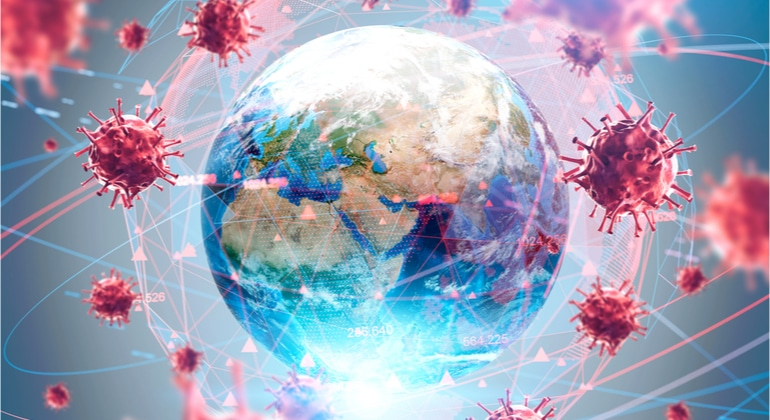
\includegraphics[width=12cm]{covid.jpg} % leia abaixo
    \caption{Pademia de Covid-19 (Foto: Shutterstock, 2020).}
    \end{figure}
	
A covid-19 é uma infecção respiratória aguda de potencial grave com números altos de mortalidade e com elevada taxa de transmissão e distribuição global. Sendo uma doença que se manifesta de formas diferentes em cada indivíduo, geralmente a maioria dos infectados desenvolve a doença em grau leve e se recuperam sem hospitalização e já em outros casos onde ela se manifesta de forma mais grave pode necessitar a hospitalização e até causar o óbito do infectado. Os principais sintomas comuns são febre, tosse, cansaço e perda do paladar e olfato; já os sintomas incomuns são dor de cabeça, diarréia, dor de garganta e olhos irritados ou vermelhos; agora os sintomas graves são dificuldade de respirar ou falta de ar, dor no peito, dificuldades para falar, confusão mental e dificuldades de locomoção.\cite{WorldHealthOrganization} Nos casos mais graves o paciente deverá receber auxílio de aparelhos respiratórios para ajudar na respiração.

No Brasil, assim como muitos lugares do mundo, algumas ações de controle de contaminação foram impostas pelas autoridades governamentais recomendadas pela OMS, são elas o uso obrigatório de máscara, o distanciamento social, a proibição de aglomerações, a correta higienização das superfícies e das mãos, toque de recolher e entre outras. Todas essas medidas foram com o intuito de frear os impactos da covid, diminuir a contaminação, evitar mortes e superlotação dos hospitais.\cite{werneck2020pandemia} Apesar de esforços de parte da população para combater a pandemia a desinformação e a negação fez com que algumas pessoas impedisse que o Brasil conseguisse reduzir os impactos negativos em nossa sociedade, o alto número de mortos, mutações do vírus e o grande número de contaminados foram alguma das consequências mais graves.
	
A Computação é uma grande aliada nessa luta contra a covid-19, os estudos em diversas partes da computação podem auxiliar na hora de entender o problema ou na hora de criar modelos de soluções. Esse trabalho tem como proposta aplicar técnicas de mineração de dados com a intuição de que a partir dos dados de covid-19 seja possível computacionalmente prever números, analisar o progresso, identificar problemas e achar soluções, tendo como principal foco relacionar as caracteristicas e sintomas em comum entre os pacientes. A partir da obtenção dos dados será aplicado o processo de KDD (Knowledge Discovery in Databases), que é um processo de descoberta de conhecimento em uma base de dados, com o objetivo de estudar esses dados. O processo de KDD consiste em usar nove passos que irão ajudar a extrair informações importantes e úteis de uma base de dados. Esses passos consistem em: compreender o domínio dos dados, selecionar e criar o conjunto de dados, pré-processar e limpar os dados, transformar os dados, realizar a previsão e descrição, escolher o algoritmo de mineração de dados, utilizar o algoritmo de mineração, avaliar os resultados e, por fim, usar o conhecimento descoberto na base.\cite{fayyad1996kdd}

\chapter{Mineração de Dados}

Desde de o inicio da computação estudar dados tem sido uma atividade bastante fundamental e com o passar do tempo isso vem se tornando cada vez mais importante e necessário, hoje podemos dizer que dados são um dos recursos computacionais mais valiosos, sendo de extrema importância para qualquer empresa ou instituição. Uma das tecnologias mais utilizadas quando se trata de estudar e explorar dados é a Mineração de Dados. 

	O termo Mineração de Dados se refere ao conjunto de técnicas utilizadas para descobrir conhecimento explorando os dados, esse processo busca encontrar padrões, irregularidades e correlações entre os dados de uma base. Cada caso exige uma estratégia de mineração diferente, cabe então ao cientista de dados escolher a técnica adequada ao seu problema, por isso é necessário conhecer bem o tipo de dado que será trabalhado. 
	
Preparar os dados é uma atividade essencial e muito importante para o processo de mineração, pois a partir da preparação dos dados poderemos inicialmente compreender melhor a natureza dos dados e assim escolher o melhor caminho para se usar. Para isso alguns passos são necessários, sendo o primeiro a limpeza dos dados onde será eliminado a inconsistência na base, como a exclusão de valores errados e incompletos, a substituição por padrões mais consistentes em alguns casos, e até mesmo o agrupamento de alguns valores. Em seguida podemos integrar alguns dados ou até mesmo bases, isso vai depender da necessidade encontrada. Outra etapa importante é a transformação dos dados, que é basicamente converte-los para uma forma que possa suprir seus objetivos estabelecidos. Por fim temos a redução de dados, parte em que se descartam dados desnecessários para o estudo.\cite{camilo2009mineraccao}

Após a preparação dos dados segue-se a mineração de dados realizando algumas tarefas importantes, como a descrição, que é a parte em que se descreve os padrões e tendências descobertos nos dados aplicando técnicas específicas de análise exploratória. Tem também a tarefa de classificação, que consiste em identificar a classe em que os dados pertencem, o que representam. Segue-se com a parte de estimação, sendo exclusiva para dados numéricos, onde se busca através do números gerar valores futuros, isso com a ajuda de algoritmos específicos, no caso de atributos não numéricos existe a predição que gera os valores desses valores. O agrupamento é outra tarefa de grande importância para a mineração, ela agrupa valores similares ou que tenha alguma complementação entre si, isso ajuda a enxergar melhor os dados. Finalizando as tarefas, tem-se a associação, que é nada mais que associar informações entre os dados, isso para construir e achar conhecimento.\cite{camilo2009mineraccao} 

Finalizando o processo de mineração é chegado o momento de se falar dos métodos, que são tecnicamente os algoritmos de mineração de dados, esses que são divididos em dois grupos, os supervisionados e os não supervisionados. A diferença entre eles é que, os supervisionados são os métodos que utilizam conjuntos de dados de resultados já pré-definidos para trabalhar a saída de informações no treinamento. Já o não supervisionado os métodos tentam entender os dados sem nenhum resultado pré definido, trabalha de forma que com os dados o algoritmo chegue a algum resultado.\cite{camilo2009mineraccao}  Existem vários algoritmos que podem ser aplicados na mineração de dados, exemplos como, árvores de decisão, redes neurais, naive bayes, algoritmos genéticos, regras de associação, entre outros, vai da necessidade e da escolha do cientista de dados. Assim, através dos métodos é esperado chegar a conclusão do estudo e exploração dos dados, sendo que pode ou não ter encontrado conhecimento com a mineração.



\chapter{Objetivos}
\subsection*{Objetivo Geral}
O objetivo geral deste projeto é estudar os dados de pacientes de Covid-19 aplicando técnicas de mineração de dados com a intenção de encontrar características em comum entre os pacientes e relacionar os sintomas de Covid-19.

\subsection*{Objetivo Específico}

Os objetivos específicos do presente projeto são: 
\begin{enumerate}
    \item Obter os dados dos pacientes Covid-19.
	\item Fazer uma analise inicial dados obtidos.
	\item Aplicar técnicas e algoritmos de mineração de dados para encontrar características e sintomas em comum entre os pacientes de Covid-19.
	\item Descobrir conhecimentos nos dados de Covid-19.
	\item Avaliar as informações descobertas.
	\item Identificar problemas e mostrar resultados.
\end{enumerate}


\chapter{Materiais e Métodos}

O principal material de estudo é a base de dados de pacientes de covid-19, dados coletados nos hospitais de todo o Brasil durante o período de fevereiro de 2020 a abril de 2021. 


	Foi escolhido para a Mineração de Dados o processo de KDD, que consiste em um processo que é a descoberta de conhecimento em uma base de dados através da aplicação de técnicas específicas que permite que seja possível obter informações importantes com os dados. A partir dos dados de pacientes de covid-19 foi usada essa técnica a fim de encontrar características e sintomas em comum entre os pacientes e assim podendo relacionar-los para a descoberta de algum conhecimento. Esse processo tem nove passos iterativos e interativos, ou seja, pode ser necessário voltar algumas etapas durante o processo para regular alguma etapa, por isso é necessário ter total conhecimento e clareza sobre todas as partes do processo. Segue-se nove passos na seguinte ordem: compreender o domínio dos dados, selecionar e criar o conjunto de dados, pré-processar e limpar os dados, transformar os dados, realizar a previsão e descrição, escolher o algoritmo de mineração de dados, utilizar o algoritmo de mineração, avaliar os resultados e, por fim, usar o conhecimento descoberto na base. \cite{maimon}
    
    \begin{figure}[h]

    \centering
    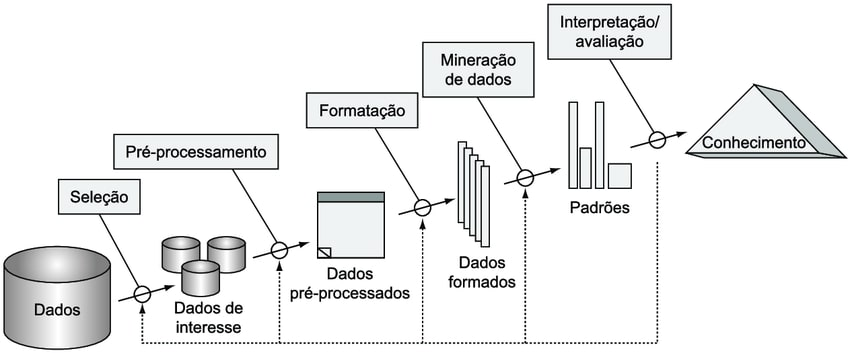
\includegraphics[width=12cm]{kdd.jpg} % leia abaixo
    \caption{Etapas do processo KDD (FAYYAD et al., 1996).}
    \end{figure}


Como não se conhece a natureza da base de dados se inicia o processo criando um dicionário de dados para o entendimento inicial das informações contidas da base de pacientes de covid-19.  O dicionário de dados é uma listagem dos elementos da base de dados de modo que fique bem definida a natureza deles. Com o dicionário de dados é possível obter várias informações sobre os dados, como tipo, tamanho, quantidade, domínio, descrição e o nome dos atributos. O dicionário de dados auxilia na análise dos dados, servindo como um ponto inicial para realizar a seleção dos dados de interesse. Com a visualização dos dados das bases fica possível ver os elementos como os atributos e entidades, assim passa ser possível fazer a limpeza dos dados descartando os elementos desnecessários ou que estão em branco, deixando apenas os mais importantes para os estudos. Realiza-se então a formatação dos dados de modo que fica mais simples e prático trabalhar com o desejado.
	
	
	Seguidamente com os dados formatados é realizada as estatísticas dos dados para que seja possível visualiza-los graficamente e assim ter uma ideai de como eles se comportam, para isso usa-se um algoritmo para gerar uma análise estatística dessa base. Pelo fato da base ser muito grande com alto volume de dados foi usado o Anaconda, que é um open source da linguagem de programação Python, para processar as informações e assim permitindo que seja possível gerar gráficos estatísticos dos dados. O Anaconda é uma ferramenta de distribuição python direcionada para área científica, especificamente para as áreas de ciência de dados, aprendizado de maquina, inteligência artificial e mineração de dados, ela permite a criação de algoritmos em python de forma direta e intuitiva. Tem uma grande distribuição de pacotes de bibliotecas específicas, aqui será escolhidas as direcionadas para manipulação dos dados e para a plotagem de gráficos estatísticos. Sendo uma delas a biblioteca Pandas que é uma ferramenta de análise e manipulação de dados de código aberto, rápida, poderosa, flexível e fácil de usar e a biblioteca matplotlib.pyplot fornece uma estrutura de plotagem de gráficos.
	
	
	K-means foi uma das escolhas de algoritmo para a mineração de dados, ele é um algoritmo de clusterização onde se separa o conjunto de dados em vários grupos diferentes a partir de vários pontos (clusters), em que cada um desses pontos é de um subgrupo. Esse algoritmo possibilita ver e achar padrões nos dados através do agrupamento sendo uma ótima escolha para o problema trabalhado, pois além de ser um grande conjunto de dados ele ainda vai possibilitar maior visualização dos pontos onde estão os problemas.\cite{kmeans} Porém no final o algoritmo escolhido foi o A Priori, pelo fato dele ser mais adequado para os dados trabalhados e para chegar nos resultados esperado. O A Priori é um algoritmo de classificação de conjuntos de itens frequentes que usa regras de associação para isso, recomendado para ser aplicado em grandes bases de dados com muitos números de transações entre os itens, ele é um ótimo algoritmo para se descobrir ou explorar padrões relevantes para estudos.\cite{agrawal1993mining}







\chapter{Análise Preliminar}

Após os dados serem selecionados e pré-processados, foram gerados alguns gráficos que permitiram a visualização da base, dessa forma foi possível analisar algumas informações contidas nos dados. Segue abaixo os gráficos gerados:

 \begin{itemize}
 \setlength{\parindent}{1.25cm}
   \item\textbf{Casos de Covid}
   \begin{figure}[h]
    \centering
    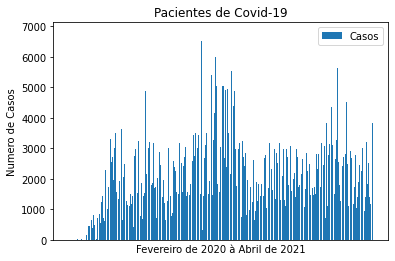
\includegraphics[width=9cm]{GBarra.png}% leia abaixo
    \caption{Gráfico de Barras dos caso de Covid-19}
    \end{figure}
    
    Esse primeiro gráfico exibe o número de casos em relação ao decorrer dos dias, com o intervalo de tempo entre fevereiro de 2020 e abril de 2021. Observa-se os períodos de maior e de menor número de casos, assim sendo possível indicificar as ondas da pandemia (intervalos de crescimento acentuado de números de casos). 
   
   \item\textbf{Perfil}
    \begin{figure}[h]
    \centering
    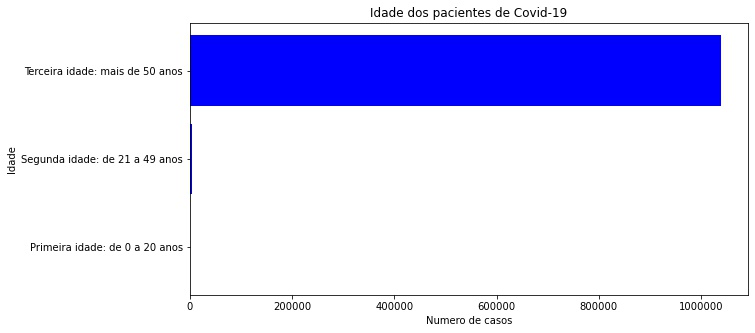
\includegraphics[width=12cm]{Idade.jpg} % leia abaixo
    \caption{Gráfico de Barras verticais da idade dos pacientes.}
    \end{figure}
    
    Agora analisando o perfil dos pacientes, vemos aqui na figura 4 o gráfico mostrando a idade dos pacientes, onde observamos que a grande maioria são da idade acima dos 50 anos, portanto confirma-se que idosos foram os mais afetados.
    
    \begin{figure}[h]
    \centering
    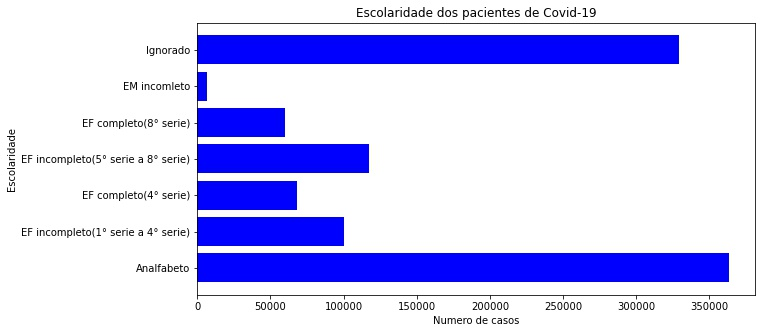
\includegraphics[width=12cm]{Escolaridade.jpg} % leia abaixo
    \caption{Gráfico de Barras verticais da escolaridade dos pacientes.}
    \end{figure}
    
    Já aqui temos a escolaridade dos pacientes, indicando que grande parte é composta por pessoas analfabetas, e que muitos tiveram seus dados escolares ignorados na ficha de cadastro. Então relacionando com a figura 4, de idade, podemos concluir que a população idosa tem um índice muito alto de analfabetismo no Brasil.

    \begin{figure}[h]
    \centering
    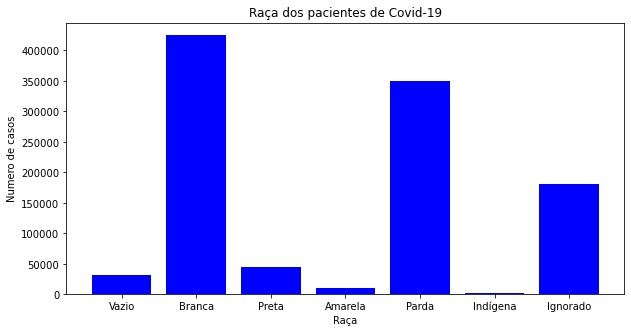
\includegraphics[width=9cm]{Raca.jpg} % leia abaixo
    \caption{Gráfico de Barras da raça dos pacientes.}
    \end{figure}
   
   Em relação as raças dos pacientes, vemos graficamente que a grande maioria dos pacientes são da raça branca seguidas da raça parda. Existe grande quantidade de pessoas que tiveram seus dados raciais ignorados. Assim concluímos que a raça branca é a que tem mais casos enquanto a preta e a indígena são as com menos.
   
   \begin{figure}[h]
    \centering
    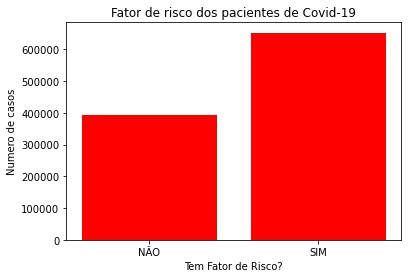
\includegraphics[width=7.3cm]{FatorRisco.jpg} % leia abaixo
    \caption{Gráfico de Barras do fator de risco dos pacientes.}
    \end{figure}
    
    O gráfico trás a questão do fator de risco, onde concluímos que a maioria dos pacientes tem alguma característica que o coloca nesse campo de risco.
   
    \begin{figure}[h]
    \centering
    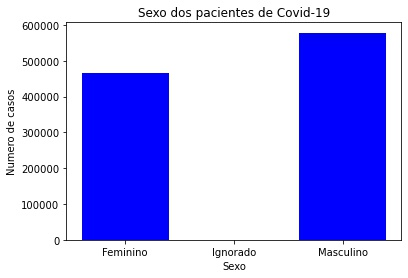
\includegraphics[width=7.3cm]{Sexo.jpg} % leia abaixo
    \caption{Gráfico de Barras do sexo dos pacientes.}
    \end{figure}
   
   Para finalizar o perfil, observamos o sexo dos pacientes, onde o gráfico mostra que entre os casos de covid-19 a maioria dos pacientes são do sexo masculino, afirmamos então que sexo feminino tem a menor taxa de pacientes.
   
  
    \item\textbf{Sintomas}
    \begin{figure}[h]
    \centering
    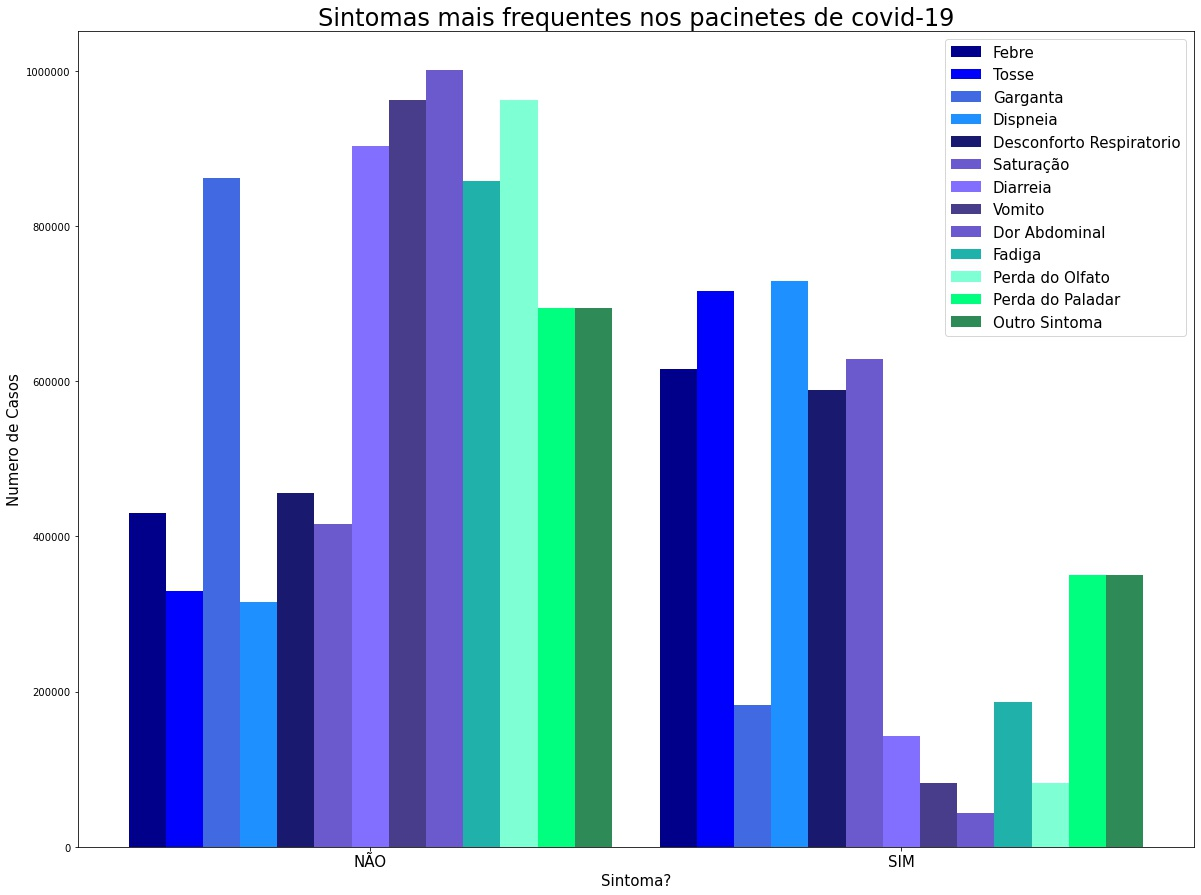
\includegraphics[width=10cm]{Sintomas.jpg} % leia abaixo
    \caption{Gráfico de Barras dos sintomas frequentes dos pacientes.}
    \end{figure}
    
    O gráfico acima mostra os sintomas mais frequentes entre os pacientes de covid-19, trazendo os casos em que os sintomas aparecem ou não. Observa-se que os sintomas mais frequentes são, em sequência, dispneia ( falta de ar ou dificuldade de respirar), tosse, saturação (quantidade de oxigênio que está circulando no sangue) e febre. Ainda vemos que existem outros sintomas que são variados, esses que aparecem em quantidade muito baixa para serem frequentes e então são colocados em uma só categoria (Outro sintoma).
 
    \item\textbf{Comorbidades}
    \begin{figure}[h]
    \centering
    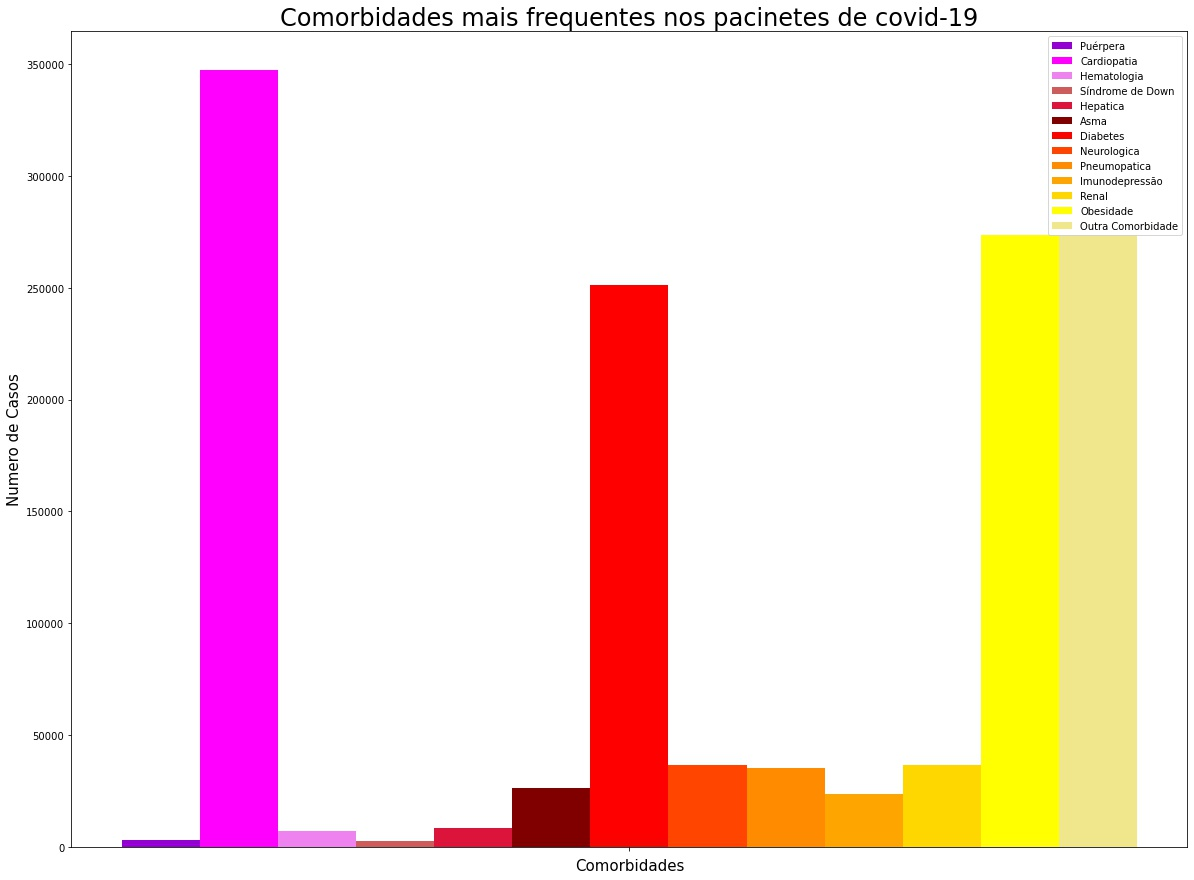
\includegraphics[width=11cm]{Comorbidade_solo.jpg} % leia abaixo
    \caption{Gráfico de Barras das comorbidades frequentes.}
    \end{figure}
    
    O gráfico trás as comorbidades que são mais comuns entre os casos de covid-19, onde podemos observar que cardiopatia é a comorbidade mais comum entre os pacientes, seguido de obesidade e diabetes. Temos também uma grande índice de variedades de outras comorbidades. 
    
 
 
 \end{itemize}


    
\chapter{Algoritmo A Priori}

O Algoritmo A Priori é um algoritmo de mineração de dados que trabalha com a ideia de conjuntos de itens frequentes, em outras palavras, ele ajuda a identificar os padrões que existem entre os dados. Desenvolvido em 1994 por R. Agrawal e R. Srikant, ele tem como objetivo encontrar conjuntos de itens frequentes em uma base de dados através de regras de associação. Regras de Associação tem como objetivo encontrar relacionamentos importantes entre grupos de itens nos dados trabalhados e exibe a frequência com que um conjunto de itens ocorre nesse processo de relacionamento.\cite{liu2010study}

\begin{itemize}
 \setlength{\parindent}{1.25cm}
 \item\textbf{Regra de Associação}
  
  Uma Regra de Associação é um método de descobrir a relação entre os itens de uma base de dados. Sabendo que uma base de dados é constituída de um conjunto de transações, temos que as transações são únicas e que cada uma é formada por um subconjunto de itens. Logo uma Regra de Associação é um relacionamento (X=>Y), sendo X e Y subconjuntos de itens, ou seja, se tem item X em um conjunto, provavelmente terá item Y também.\cite{agrawal1993mining}
  
  Para chegar em regras que sejam pertinentes para a base de dados são utilizados alguns cálculos específicos, que são eles, medidas de  Suporte(Support), Confiança(Confidence) e Aumento(Lift).
    \begin{figure}[!h]
    \centering
    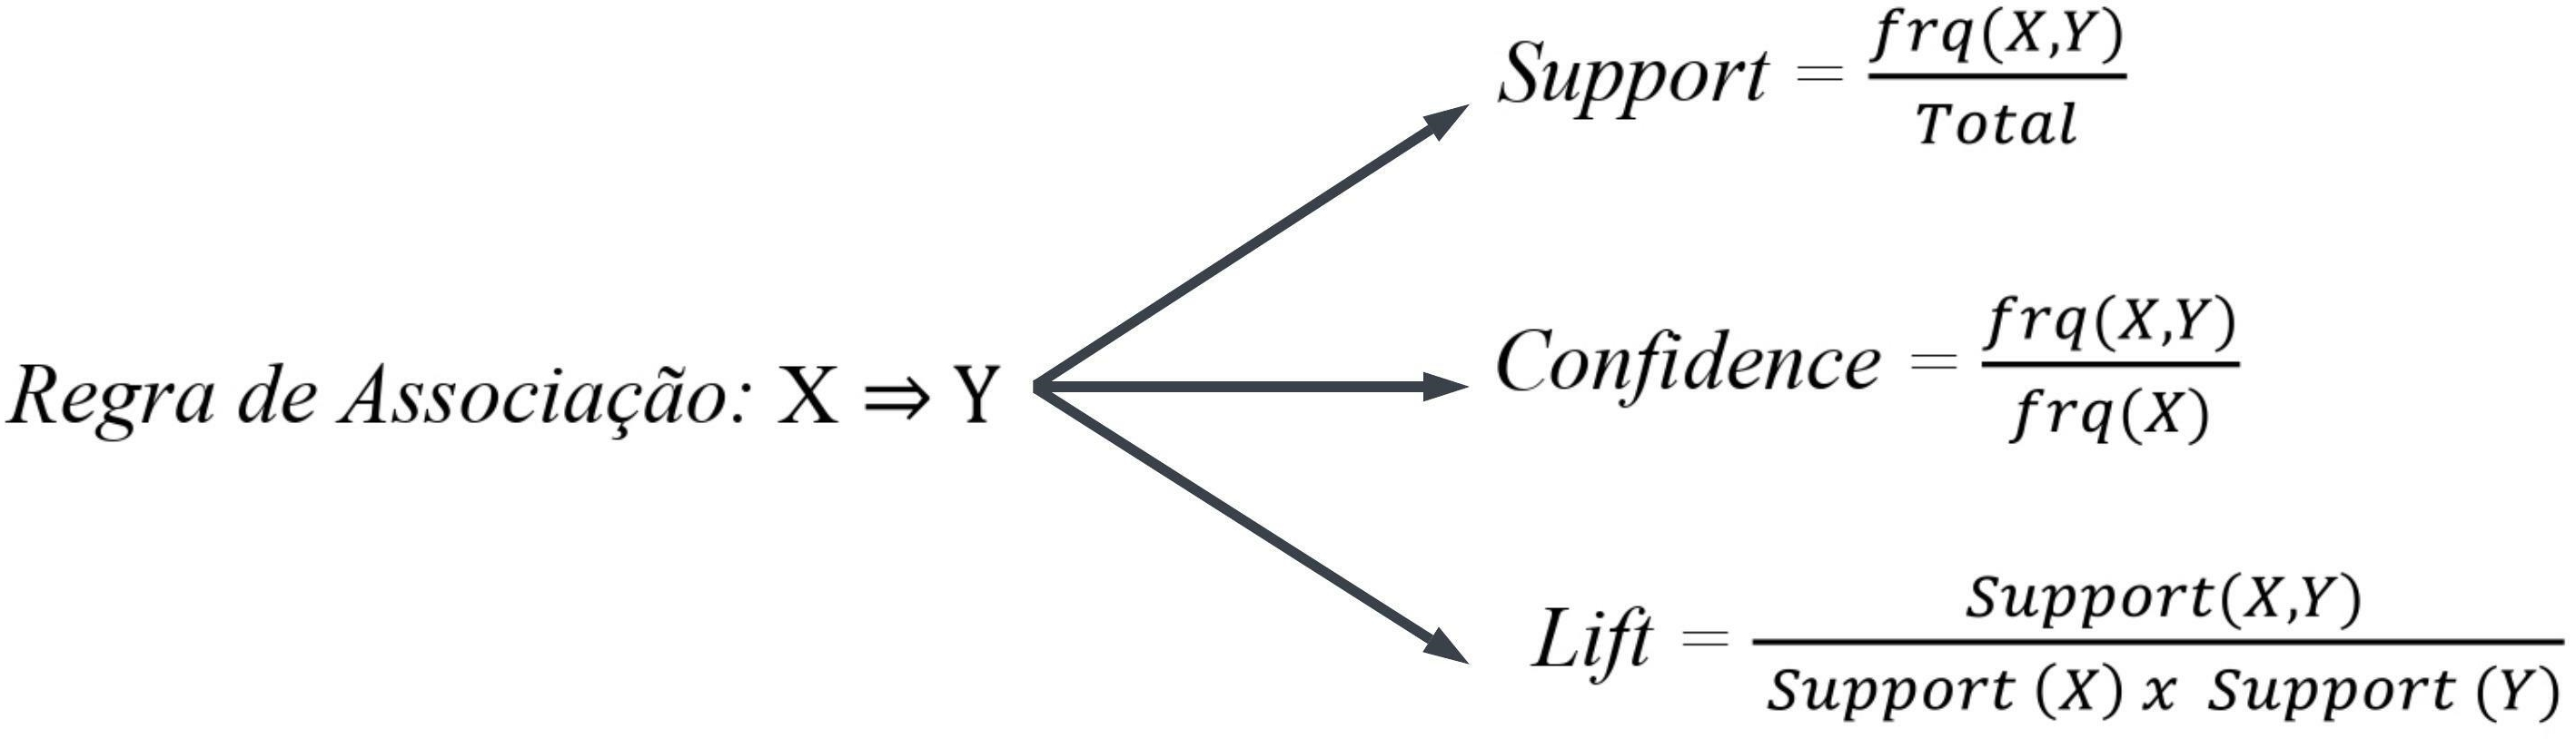
\includegraphics[width=12cm]{formula_000.jpeg}
    \end{figure}
    \begin{description}
    \item[Support:] é a proporção de um valor ou valores N na base de dados, ou seja, a frequência em que um determinado item ou itens aparecem no conjunto de dados. 
    \item[Confidence:] é o valor que informa a porcentagem de ocorrências em que a Regra de Associação é verdadeira, que é basicamente a frequência em que itens N aparecem juntos e associados em um conjunto. 
    \item[Lift:] é o valor que informa qual é o grau de associação entre os itens conjunto. Se o valor do lift for igual a 1 significa que os itens são independentes e não existe relação entre eles, se for acima de 1 os itens estão fortemente relacionados e se for menor que um os itens estão relacionados fracamente. 
    \end{description}

 \end{itemize}

A escolha do nome  A Priori para o algoritmo foi pelo fato dele usar o conhecimento prévio das propriedades frequentes do conjunto de itens, sabendo que a expressão A priori é utilizada no cotidiano com a finalidade de realizar menção a um motivo anterior à experiência. Na execução aplicamos uma abordagem iterativa ou busca em nível a onde conjuntos de itens k-frequentes são usados para encontrar conjuntos de itens k+1. 

Com a intenção de aprimorar a eficiência da geração de conjuntos de itens frequentes, uma propriedade essencial é usada, que é nomeada de propriedade Apriori, que auxilia a reduzir o zona de busca.


 \begin{itemize}
 \setlength{\parindent}{1.25cm}
 \item\textbf{Propriedade Apriori}
  
  A propriedade Apriori afirma que, todo subconjunto não vazio do conjunto de itens frequente deve ser frequente. A definição base do algoritmo Apriori é sua anti-monotonicidade do valor de suporte. O algoritmo assume que todos os subconjuntos de um conjunto de itens frequente devem ser frequentes. Se um conjunto de itens for infrequente, todos os seus superconjuntos serão infrequentes.
 
 \end{itemize}

Explicando agora o funcionamento e os passos do algoritmo será usado um conjunto de dados como exemplo que servirá como suporte para melhor entendimento. Esses dados se tratam de um lista de clientes de uma barraca de hortifrútis de uma feira, onde mostra os itens comprados por cada um desses clientes. 
    \begin{figure}[h]
    \centering
    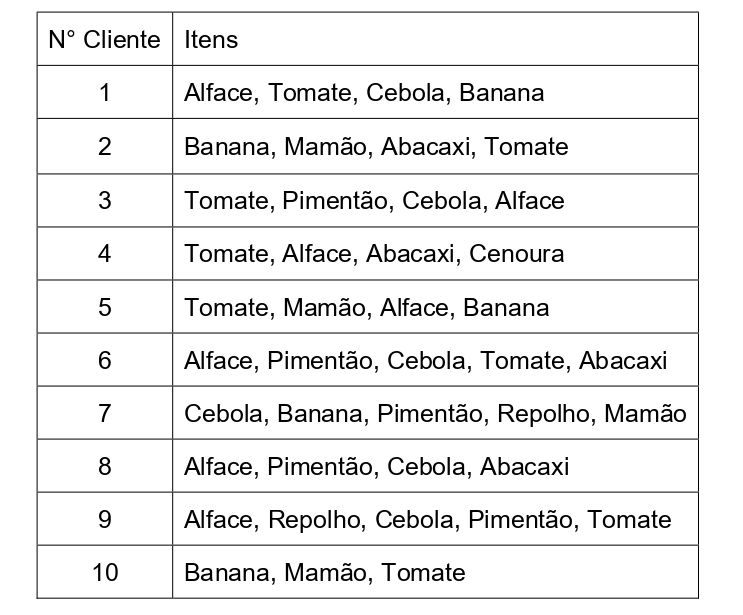
\includegraphics[width=8cm]{tabela de clientes.jpg}
    \end{figure}
    
Observando a base de dados vemos que ela é composta por duas colunas, onde a primeira é o numero do cliente e a segunda os produtos/itens comprados por cada um deles. Então o primeiro passo do A Priori vai ser calcular de forma individual o suporte de cada item da base, que vai ser basicamente contar o numero de ocorrências de um determinado produto e dividir pelo valor total, para isso utiliza-se a formula de suporte apresentada anteriormente, adaptando ao primeiro passo a formula será a seguinte, onde X é o item selecionado: \textit{Support=}${\frac{frq(X)}{Total}}$.
    
Assim geramos a tabela a seguir com o numero de suporte de cada produto. 
    \begin{figure}[h]
    \centering
    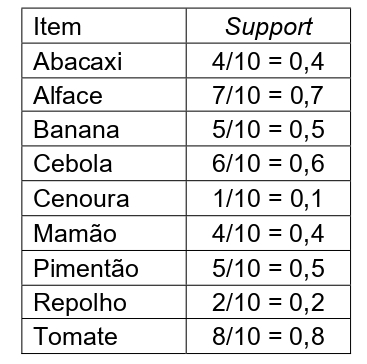
\includegraphics[width=5cm]{passo_1.jpg}
    \end{figure}

Depois de calcular o suporte de cada item X, passamos para o segundo passo, que é escolher o suporte mínimo para filtrar os itens que não são frequentes. Vamos escolher então para o exemplo trabalhado o peso 0,5 como critério de filtragem. Seguindo para o passo três, iremos usar o suporte mínimo e fazer a filtragem dos itens, logo temos os itens mais frequentes abaixo.
    \begin{figure}[h]
    \centering
    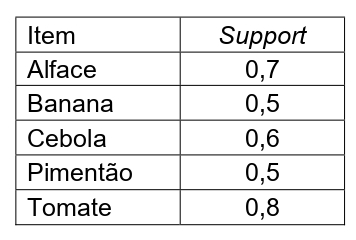
\includegraphics[width=5cm]{passo_2.jpg}
    \end{figure}

Indo para o quarto passo, será calculado novamente o suporte, mas agora para o conjunto de combinações de itens. Essa combinação é através das formações de pares de todos os itens do conjunto trabalhado, lembrando de ignorar as combinações onde aparecem itens não frequentes, esses que foram descartados pela filtragem. Após a combinação foi realizado o calculo de suporte novamente, agora adaptando a formula para dois itens (X e Y), a formulá ficara assim:  \textit{Support=}${\frac{frq(X,Y)}{Total}}$.

Passando para o próximo passo, é feita a filtragem novamente com o suporte mínimo de 0,5 gerando assim um novo conjunto. Vemos então abaixo as duas tabelas geradas nessas duas etapas, sendo a primeira o resultado das combinações e o calculo de suporte dos itens e a segunda a filtragem com o suporte mínimo.
    \begin{figure}[!h]
    \centering
    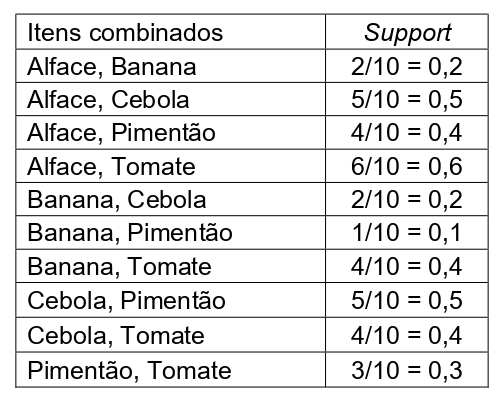
\includegraphics[width=6cm]{passo_3.jpg}
    
\includegraphics[width=1cm]{seta.png}
    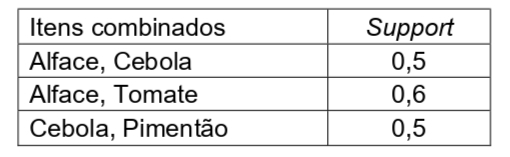
\includegraphics[width=6cm]{passo_4.jpg}
    \end{figure}

No sexto passo é repetido processo para combinações, só que agora entre três itens, lembrando de descartar as duplas não frequentes para formar os trios chegamos as combinações e já é feito novamente o calculo de suporte, adaptando a formula para três tipos de itens, sendo a seguinte formula:  \textit{Support=}${\frac{frq(X,Y,Z)}{Total}}$. Chegamos aos seguintes conjuntos de trios abaixo com seus suportes calculados.
    \begin{figure}[!h]
    \centering
    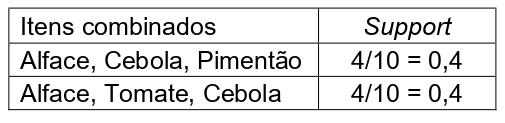
\includegraphics[width=6cm]{passo_5.jpg}
    \end{figure}

Filtrando os trios de conjuntos onde o desejado é que suporte mínimo seja de 0,5, descartamos todos os dois trios, já que eles tem o suporte 0,4. Então prosseguimos os passos do algoritmo com os conjuntos de duplas apresentados anteriormente, pous apresentam o suporte mínimo desejado.
    \begin{figure}[!h]
    \centering
    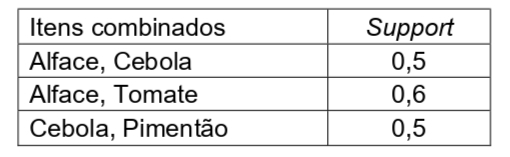
\includegraphics[width=6cm]{passo_4.jpg}
    \end{figure}

O próximo e ultimo passo do algoritmo A Priore é criar as Regras de Associação e calcular a confiança e o lift dos conjuntos. 
    \begin{figure}[!h]
    \centering
    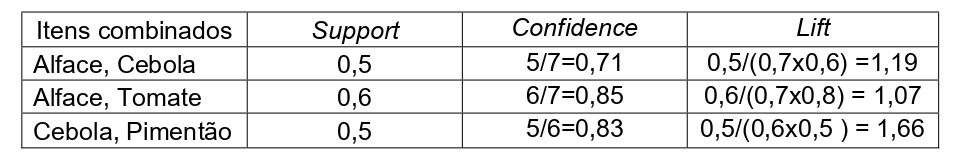
\includegraphics[width=13cm]{final_1.jpg}
    \end{figure}

Finalizando o algoritmo temos o seguinte resultado:
    \begin{figure}[!h]
    \centering
    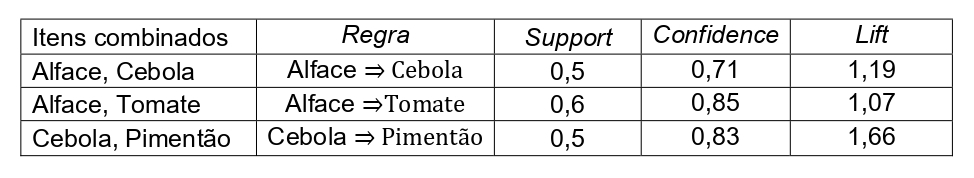
\includegraphics[width=13cm]{final_2.jpg}
    \end{figure}

Com o algoritmo A Priori chegamos á alguns resultados a cerca da base de dados da barraca de hortifrúti da feira, sendo eles que:
 \begin{itemize}
   \item 50\% dos clientes que compraram alface levaram cebola;
   
   A confiança de uma pessoa que compre alface levar cebola é de 71\%.
   \item 60\% dos clientes que compraram alface levaram tomate;
   
   A confiança de uma pessoa que compre alface levar tomate é de 85\%.
   \item 50\% dos clientes que compraram cebola levaram pimentão;
   
   A confiança de uma pessoa que compre cebola levar pimentão é de 83\%.
 \end{itemize}

\chapter{Resultados - Aplicando o algoritmo de mineração A Priori no dados de Covid-19}

 Escolher o algoritmo de mineração de dados foi uma tarefa desafiadora, já que existe uma variedade muito grande de algoritmos e poucos apenas que podem funcionar nos dados trabalhados, por isso nesse momento é preciso saber escolher o que mais vai gerar resultados consistentes e uteis para o estudo. Após a formatação e uma analise profunda dos dados e dos gráficos gerados concluiu-se que o A Priori seria o mais adequado para a base trabalhada pois ele funciona com a ideia de itens frequentes e como a intenção principal aqui é relacionar as caraterísticas dos pacientes deu muito certo. 
 
 A implementação do algoritmo foi feita em Python utilizando a plataforma Anaconda que disponibiliza varias bibliotecas importantes e uteis para trabalhar com data mining. Instalando o pacote do A Priori é só adequar os dados para serem treinados no algoritmo, assim após fazer a separação dos dados foram treinamos cada grupo separados da base de dados e chegamos a alguns resultados interessantes que serão mostrados a seguir.

 \begin{itemize}
   \item\textbf{Sintomas}
   \setlength{\parindent}{1.2cm}
   
   O primeiro resultado trás o algoritmo aplicado aos dados de sintomas dos pacientes de covid-19, após a separação dos dados e uma analise dos gráficos de frequência foi escolhido o valor de 0.45 para ser o suporte mínimo para a filtragem do algoritmo, temos como resultado a figura 11. 
   
    \begin{figure}[!h]
    \centering
    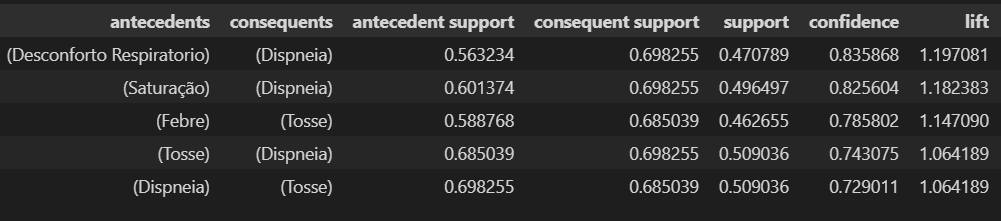
\includegraphics[width=15cm]{resultado_apriori_01.png} % leia abaixo
    \caption{Resultado do algoritmo A Priori treinado com os dados de sintomas dos pacientes de covid-19 }
    \end{figure}
    
    Analisando o resultado vemos que encontramos 5 regras de associação para os sintomas, sendo elas: 
    \textbf{Desconforto respiratório => Dispneia} com o support igual a 0.470789, confidence 0.835868 e o lift de 1.197081;
    \textbf{Saturação => Dispneia} com o support igual a 0.496497, confidence 0.825604 e o lift de 1.182383; 
    \textbf{Febre => Tosse} com o support igual a 0.462655, confidence 0.785802 e o lift de 1.147090;
    \textbf{Tosse => Dispneia} com o support igual a 0.509036, confidence 0.743075 e o lift de 1.064189;
    \textbf{Dispneia => Tosse} com o support igual a 0.509036, confidence 0.729011 e o lift de 1.064189.
    
    
    Separando os pacientes por sexo (Feminino e Masculino) descartando os que não informaram o sexo, temos os dois resultados mostrados respectivamente nas figuras 12 e 13 onde o suporte continua com mínimo de 0.45 pois esse valor está sendo adequado para alcançar resultados desejados com esse grupo de dados separado da base de dados.
    \begin{figure}[!h]
    \centering
    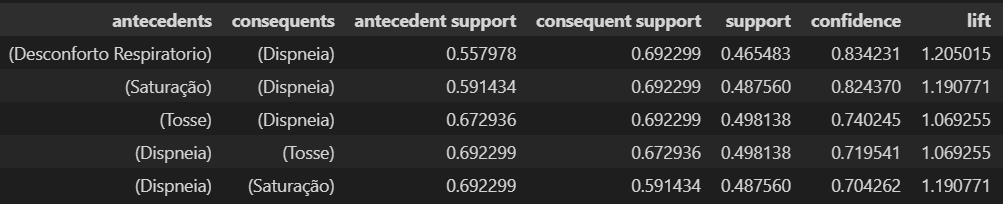
\includegraphics[width=15cm]{resultado_apriori_02(sexoFeminino).png} % leia abaixo
    \caption{Resultado do algoritmo A Priori treinado com os dados de sintomas de covid-19 dos pacientes do sexo feminino}
    \end{figure}
    
    Analisando o resultado dos pacientes do sexo feminino encontramos 5 regras de associação para os sintomas, sendo elas: 
    \textbf{Desconforto respiratório => Dispneia} com o support igual a 0.465483, confidence 0.834231 e o lift de 1.205015;
    \textbf{Saturação => Dispneia} com o support igual a 0.487560, confidence 0.824370 e o lift de 1.190771; 
    \textbf{Tosse => Dispneia} com o support igual a 0.498138, confidence 0.740245 e o lift de 1.069255;
    \textbf{Dispneia => Tosse} com o support igual a 0.498138, confidence 0.719541 e o lift de 1.069255;
    \textbf{Dispneia => Saturação} com o support igual a 0.487560, confidence 0.704262 e o lift de 1.190771.
    
    
    \begin{figure}[!h]
    \centering
    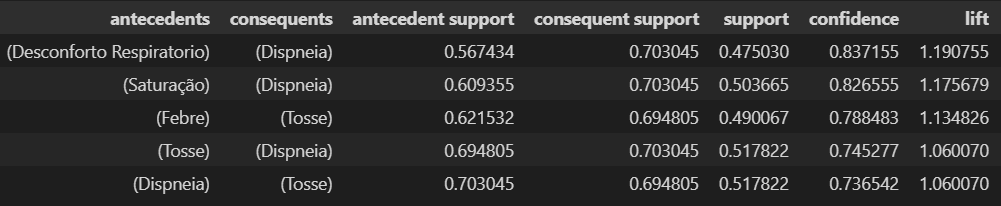
\includegraphics[width=15cm]{resultado_apriori_03(sexoMasculino).png} % leia abaixo
    \caption{Resultado do algoritmo A Priori treinado com os dados de sintomas de covid-19 dos pacientes do sexo masculino}
    \end{figure}
    
    Agora o resultado dos pacientes do sexo masculino onde encontramos 5 regras de associação para os sintomas, sendo elas: 
    \textbf{Desconforto respiratório => Dispneia} com o support igual a 0.475030, confidence 0.837155 e o lift de 1.190755;
    \textbf{Saturação => Dispneia} com o support igual a 0.503665, confidence 0.826555 e o lift de 1.175679; 
    \textbf{Febre => Tosse} com o support igual a 0.490067, confidence 0.788483 e o lift de 1.134826;
    \textbf{Tosse => Dispneia} com o support igual a 0.517822, confidence 0.745277 e o lift de 1.060070;
    \textbf{Dispneia => Tosse} com o support igual a 0.517822, confidence 0.736542 e o lift de 1.060070.
    
    Separando aqui os pacientes por raça, sendo que após uma analise dos dados e dos gráficos foi decidido apenas selecionar os pacientes das raças Preta, Parda e Branca pois são as três mais frequentes no conjunto de dados, ainda descartando os pacientes que não teve suas raças declaradas no registro do caso de covid-19, ainda utilizando o suporte mínimo de 0.45 temos tês resultados apresentados nas figuras 14, 15 e 16.  
    

    \begin{figure}[!h]
    \centering
    \includegraphics[width=15cm]{resultado_apriori_raça_Preta.png} % leia abaixo
    \caption{Resultado do algoritmo A Priori treinado com os dados de sintomas de covid-19 dos pacientes da raça Preta}
    \end{figure}
    
    Observando os pacientes da raça preta encontramos 5 regras de associação para os sintomas, sendo elas: 
    \textbf{Desconforto respiratório => Dispneia} com o support igual a 0.494266, confidence 0.837228 e o lift de 1.182443;
    \textbf{Saturação => Dispneia} com o support igual a 0.518652, confidence 0.828845 e o lift de 1.170603; 
    \textbf{Febre => Tosse} com o support igual a 0.457753, confidence 0.797978 e o lift de 1.155071;
    \textbf{Desconforto respiratório => Saturação} com o support igual a 0.462806, confidence 0.783939 e o lift de 1.252794;
    \textbf{Tosse => Dispneia} com o support igual a 0.524122, confidence 0.758666 e o lift de 1.071487.
    
    \begin{figure}[!h]
    \centering
    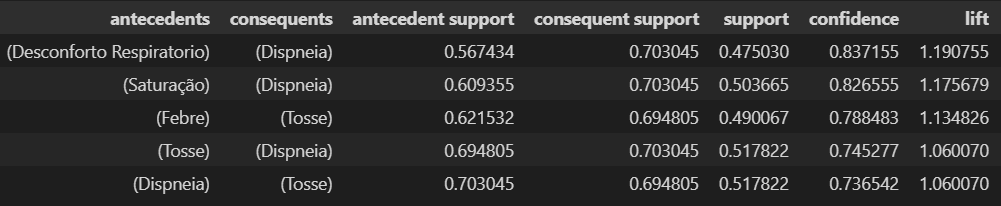
\includegraphics[width=15cm]{resultado_apriori_03(sexoMasculino).png} % leia abaixo
    \caption{Resultado do algoritmo A Priori treinado com os dados de sintomas de covid-19 dos pacientes da raça Parda}
    \end{figure}
    
    Agora o resultado dos pacientes da raça Parda onde encontramos 5 regras de associação para os sintomas, sendo elas: 
    \textbf{Saturação => Dispneia} com o support igual a 0.496941, confidence 0.844738 e o lift de 1.183988;
    \textbf{Desconforto Respiratório => Dispneia} com o support igual a 0.499082, confidence 0.842438 e o lift de 1.180764; 
    \textbf{Febre => Tosse} com o support igual a 0.494346, confidence 0.806533 e o lift de 1.145841;
    \textbf{Saturação => Desconforto Respiratório} com o support igual a 0.451869, confidence 0.768121 e o lift de 1.296568;
    \textbf{Desconforto Respiratório => Saturação} com o support igual a 0.451869, confidence 0.762743 e o lift de 1.296568.
    
    \begin{figure}[!h]
    \centering
    \includegraphics[width=15cm]{resultado_apriori_raça_Branca.png} % leia abaixo
    \caption{Resultado do algoritmo A Priori treinado com os dados de sintomas de covid-19 dos pacientes da raça Branca}
    \end{figure}
    
    Nos dados de pacientes da raça Branca encontramos também 5 regras de associação para os sintomas, sendo elas: 
    \textbf{Desconforto respiratório => Dispneia} com o support igual a 0.493476, confidence 0.840135 e o lift de 1.184520;
    \textbf{Saturação => Dispneia} com o support igual a 0.531090, confidence 0.824482 e o lift de 1.162451; 
    \textbf{Desconforto respiratório => Saturação} com o support igual a 0.466238, confidence 0.793763 e o lift de 1.232266;
    \textbf{Dispneia => Saturação} com o support igual a 0.531090, confidence 0.748791 e o lift de 1.162451;
    \textbf{Tosse => Dispneia} com o support igual a 0.511001, confidence 0.746281 e o lift de 1.052193.
    
    Indo mais a fundo nos dados foi feita a seleção dos grupos levando em consideração o sexo e a raça, assim como anteriormente apenas as raças Preta, Pardas e Branca foram selecionadas para o treinamento do A Priori, pacientes do sexo feminino das raças preta, parda e branca, e pacientes do sexo masculino das raças preta, parda e branca,  os resultados estão nas figuras 17, 18, 19, 20, 21 e 22, ainda com o suporte mínimo de 0.45.
    
    \begin{figure}[!h]
    \centering
    \includegraphics[width=15cm]{result_raçaPreta_sexoFeminino.png} % leia abaixo
    \caption{Resultado do algoritmo A Priori treinado com os dados de sintomas de covid-19 dos pacientes do sexo feminino e da raça preta}
    \end{figure}
    
    Observa-se no resultado do grupo de pacientes do sexo feminino e raça preta 5 regras de associação para os sintomas, sendo elas: 
    \textbf{Desconforto respiratório => Dispneia} com o support igual a 0.493839, confidence 0.842546 e o lift de 1.185571;
    \textbf{Saturação => Dispneia} com o support igual a 0.519660, confidence 0.832756 e o lift de 1.171795; 
    \textbf{Desconforto respiratório => Saturação} com o support igual a 0.458495, confidence 0.782245 e o lift de 1.253548;
    \textbf{Tosse => Dispneia} com o support igual a 0.518040, confidence 0.765265 e o lift de 1.076826;
    \textbf{Saturação => Desconforto Respiratório} com o support igual a 0.458495, confidence 0.734739 e o lift de 1.253548.
    
    \begin{figure}[!h]
    \centering
    \includegraphics[width=14cm]{result_raçaParda_sexoFeminino.png} % leia abaixo
    \caption{Resultado do algoritmo A Priori treinado com os dados de sintomas de covid-19 dos pacientes do sexo feminino e da raça parda}
    \end{figure}
    
    O resultado do grupo dos pacientes do sexo feminino e raça parda trás 5 regras de associação para os sintomas, elas são: 
    \textbf{Saturação => Dispneia} com o support igual a 0.485893, confidence 0.843387 e o lift de 1.194963;
    \textbf{Desconforto respiratório => Dispneia} com o support igual a 0.491113, confidence 0.839683 e o lift de 1.189715 ; 
    \textbf{Febre => Tosse} com o support igual a 0.465176, confidence 0.803692 e o lift de 1.159084;
    \textbf{Tosse => Dispneia} com o support igual a 0.522108, confidence 0.752983 e o lift de 1.066873;
    \textbf{Dispneia => Tosse} com o support igual a 0.522108, confidence 0.739754 e o lift de 1.066873.
    
    \begin{figure}[!h]
    \centering
    \includegraphics[width=14cm]{result_raçaBranca_sexoFeminino.png} % leia abaixo
    \caption{Resultado do algoritmo A Priori treinado com os dados de sintomas de covid-19 dos pacientes do sexo feminino e da raça branca}
    \end{figure}
    
    Passando para o resultado do grupo de pacientes do sexo feminino e raça branca entramos 5 regras de associação para os sintomas, elas são:
    \textbf{Desconforto respiratório => Dispneia} com o support igual a 0.488581, confidence 0.838561 e o lift de 1.189783;
    \textbf{Saturação => Dispneia} com o support igual a 0.523211, confidence 0.822305 e o lift de 1.166718; 
    \textbf{Desconforto respiratório => Saturação} com o support igual a 0.459171, confidence 0.788084 e o lift de 1.238594;
    \textbf{Tosse => Dispneia} com o support igual a 0.500715, confidence 0.744771 e o lift de 1.056710;
    \textbf{Dispneia => Tosse} com o support igual a 0.523211, confidence 0.742352 e o lift de 1.166718.
    
    \begin{figure}[!h]
    \centering
    \includegraphics[width=14cm]{result_raçaPreta_sexoFeminino.png} % leia abaixo
    \caption{Resultado do algoritmo A Priori treinado com os dados de sintomas de covid-19 dos pacientes do sexo masculino e da raça preta}
    \end{figure}
    
    Observa-se na figura 20 o resultado do grupo de pacientes do sexo masculino e raça preta 5 regras de associação para os sintomas, sendo elas: 
    \textbf{Desconforto respiratório => Dispneia} com o support igual a 0.494534, confidence 0.832943 e o lift de 1.179901;
    \textbf{Saturação => Dispneia} com o support igual a 0.517829, confidence 0.825632 e o lift de 1.169545; 
    \textbf{Febre => Tosse} com o support igual a 0.484914, confidence 0.803187 e o lift de 1.143999;
    \textbf{Desconforto Respiratório => Saturação} com o support igual a 0.466269, confidence 0.785336 e o lift de 1.252148;
    \textbf{Tosse => Dispneia} com o support igual a 0.529040, confidence 0.753525 e o lift de 1.067401.
    
    \begin{figure}[!h]
    \centering
    \includegraphics[width=14cm]{result_raçaParda_sexoFeminino.png} % leia abaixo
    \caption{Resultado do algoritmo A Priori treinado com os dados de sintomas de covid-19 dos pacientes do sexo masculino e da raça parda}
    \end{figure}
    
    O resultado do grupo dos pacientes do sexo masculino e raça parda trás 5 regras de associação para os sintomas, elas são: 
    \textbf{Saturação => Dispneia} com o support igual a 0.505627, confidence 0.845745 e o lift de 1.175427;
    \textbf{Desconforto respiratório => Dispneia} com o support igual a 0.505325, confidence 0.844559 e o lift de 1.173779; 
    \textbf{Febre => Tosse} com o support igual a 0.517435, confidence 0.808558 e o lift de 1.135321;
    \textbf{Saturação => Desconforto Respiratório} com o support igual a 0.460195, confidence 0.769752 e o lift de 1.286501;
    \textbf{Desconforto Respiratório => Saturação} com o support igual a 0.460195, confidence 0.769133 e o lift de 1.286501.
    
    \begin{figure}[!h]
    \centering
    \includegraphics[width=14cm]{result_raçaBranca_sexoFeminino.png} % leia abaixo
    \caption{Resultado do algoritmo A Priori treinado com os dados de sintomas de covid-19 dos pacientes do sexo masculino e da raça branca}
    \end{figure}
    
    Enfim por ultimo temos o resultado do grupo de pacientes do sexo masculino e raça branca entramos 5 regras de associação para os sintomas, elas são:
    \textbf{Desconforto respiratório => Dispneia} com o support igual a 0.497536, confidence 0.841424 e o lift de 1.180165;
    \textbf{Saturação => Dispneia} com o support igual a 0.537620, confidence 0.826241 e o lift de 1.158870; 
    \textbf{Desconforto respiratório => Saturação} com o support igual a 0.472101, confidence 0.798409 e o lift de 1.227037;
    \textbf{Febre => Tosse} com o support igual a 0.473676, confidence 0.781118 e o lift de 1.123790;
    \textbf{Dispneia => Saturação} com o support igual a 0.537620, confidence 0.754055 e o lift de 1.158870;
    
   \item\textbf{Comorbidades}
   
   Vindo agora para os dados de comorbidades chegamos a uma questão, que é a quantidade de dados, se tem pouco sobre as comorbidades, sendo que sua presença é bem baixa nos casos, assim dificultando alguma analise mais profunda dos dados. Porem usando um valor bem baixo de suporte o algoritmo chegou a um resultado que será mostrado na figura 23, o suporte mínimo foi de 0.10.
   
   \begin{figure}[!h]
    \centering
    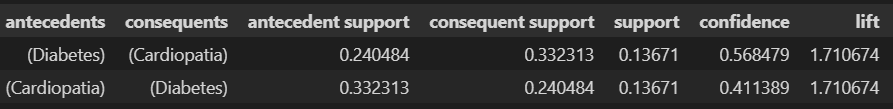
\includegraphics[width=14cm]{resultado_apriori_comorbidade.png} % leia abaixo
    \caption{Resultado do algoritmo A Priori treinado com os dados de comorbidade dos pacientes de covid-19}
    \end{figure}
   
   Temos então duas regras, que são:
   \textbf{Diabetes => Cardiopatia} com o support igual a 0.13671, confidence 0.568479 e o lift de 1.710674;
    \textbf{Cardiopatia => Diabetes} com o support igual a 0.13671, confidence 0.411389 e o lift de 1.710674; 
   
 \end{itemize}

\chapter{Conclusões}
    
    Com os resultados foi possível chegar em algumas conclusões bastante interessantes acerca dos dados da base, principalmente a relação entre os sintomas e as características dos pacientes de covid-19, que foi o foco deste projeto.
    
    Através dos gráficos estatísticos dos dados chegamos em alguns pontos importantes, que são, a maioria dos pacientes são pessoas idosas; que os incidente de casos foram maiores em pessoas do sexo masculino e de raça branca; que dispneia, tosse, saturação e febre foram os sintomas que mais ocorreram; e por ultimo que pessoas com comorbidades do tipo obesidade e diabética tiveram maior vulnerabilidade.
    
    Para finalizar temos os gráficos que mostra os conhecimentos descobertos. Primeiro temos as relações entre os sintomas descobertas através do A Priori. 

    \begin{figure}[!h]
    \centering
    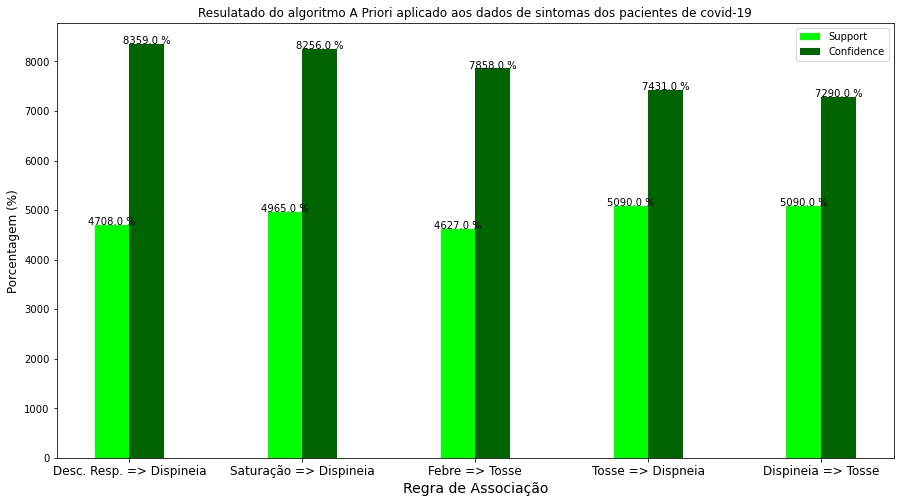
\includegraphics[width=13cm]{AprioriIMG.jpg}
    \caption{Gráfico com o resultado do A Priori aplicado aos sintomas de covid-19}
    \end{figure}
    
    \begin{itemize}
    \item 47,08\% dos pacientes que tiveram desconforto respiratório manifestaram também dispneia, sendo a confiança dessa regra acorrer de 83,59\%;
    
    \item 49,65\% dos pacientes que tiveram saturação manifestaram também dispneia, sendo a confiança dessa regra acorrer de 82,56\%;
    
    \item 46,27\% dos pacientes que tiveram febre manifestaram também tosse, sendo a confiança dessa regra acorrer de 78,58\%;
    
    \item 50,9\% dos pacientes que tiveram tosse manifestaram também dispneia, sendo a confiança dessa regra acorrer de 74,31\%;
    
    \item 50,9\% dos pacientes que tiveram dispneia manifestaram também tosse, sendo a confiança dessa regra acorrer de 72,9\%;
    \end{itemize}
    
    O maior índice de ocorrência de dois sintomas relacionados é de que pessoas que tiveram tosse também apresentaram dispneia, mas com a confiança podemos afirmar que a associação mais garantida entre os sintomas é que o paciente que tiver desconforto respiratório certamente terá dispneia.
    
    Agora relacionando o sexo dos pacientes com os sintomas.
    
    \begin{figure}[!h]
    \centering
    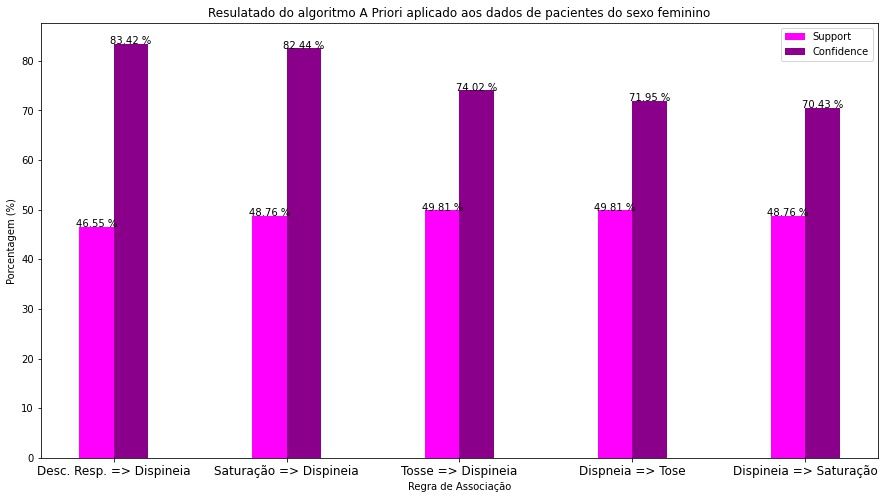
\includegraphics[width=12cm]{AprioriIMG_sexo_feminino.jpg}
    \caption{Resultado gráfico do A Priori relacionando os sintomas ao sexo feminino}
    \end{figure}
    
    \begin{itemize}
    \item 46,55\% dos pacientes do sexo feminino que tiveram desconforto respiratório manifestaram também dispneia, sendo a confiança dessa regra acorrer de 83,42\%;
    
    \item 48,76\% dos pacientes do sexo feminino que tiveram saturação manifestaram também dispneia, sendo a confiança dessa regra acorrer de 82,44\%;
    
    \item 49,81\% dos pacientes do sexo feminino que tiveram tosse manifestaram também dispneia, sendo a confiança dessa regra acorrer de 74,02\%;
    
    \item 49,81\% dos pacientes do sexo feminino que tiveram dispneia manifestaram também tosse, sendo a confiança dessa regra acorrer de 71,95\%;
    
    \item 48,76\% dos pacientes do sexo feminino que tiveram dispneia manifestaram também saturação, sendo a confiança dessa regra acorrer de 70,43\%;
    \end{itemize}
    
      O maior índice de ocorrência de dois sintomas relacionados entre os pacientes do sexo feminino é que quem tiver tosse também apresentaram dispneia, mas com a confiança podemos afirmar que a associação mais provável de ocorrer entre os sintomas é que o paciente que tiver desconforto respiratório certamente terá dispneia.
    
    \begin{figure}[!h]
    \centering
    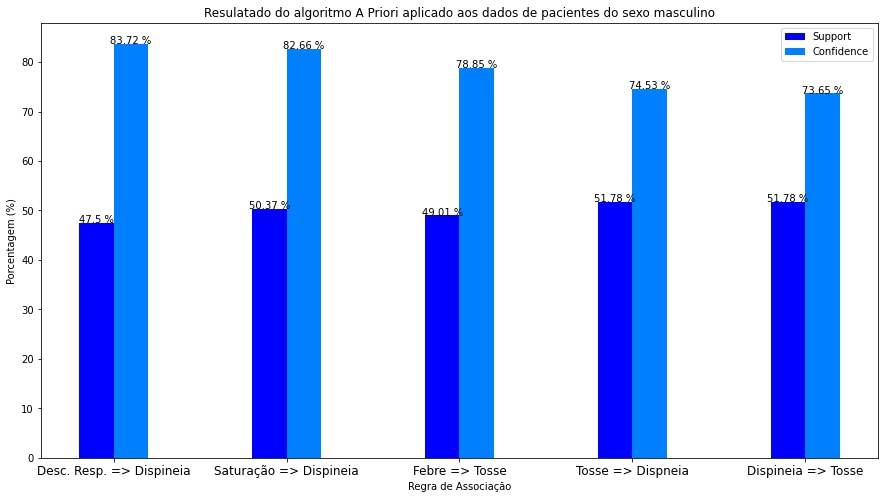
\includegraphics[width=13cm]{AprioriIMG_sexo_masculino.jpg}
    \caption{Resultado gráfico do A Priori relacionando os sintomas ao sexo masculino}
    \end{figure}
    
     \begin{itemize}
    \item 47,5\% dos pacientes do sexo masculino que tiveram desconforto respiratório manifestaram também dispneia, sendo a confiança dessa regra acorrer de 83,72\%;
    
    \item 50,37\% dos pacientes do sexo masculino que tiveram saturação manifestaram também dispneia, sendo a confiança dessa regra acorrer de 82,66\%;
    
    \item 49,01\% dos pacientes do sexo masculino que tiveram febre manifestaram tosse, sendo a confiança dessa regra acorrer de 78,85\%;
    
    \item 51,78\% dos pacientes do sexo masculino que tiveram tosse manifestaram dispneia, sendo a confiança dessa regra acorrer de 74,53\%;
    
    \item 51,78\% dos pacientes do sexo masculino que tiveram dispneia manifestaram também tosse, sendo a confiança dessa regra acorrer de 73,65\%;
    \end{itemize}
    
      Entre os pacientes do sexo masculino a associação que teve maior índice de ocorrência foi a quem teve tosse também manifestou dispneia e valendo também para a associação ao contrario (dispneia=>tosse), porém quando olhamos para a confiança podemos afirmar que a associação mais garantida de ocorrer entre os relacionamentos é a de que se o paciente do sexo masculino tiver desconforto respiratório certamente terá dispneia também, assim como nos pacientes de sexo feminino.
      
      Logo podemos dizer acerca dos dados apresentados que o sexo tem pouca influencia nas relações entre sintomas, só se pode afirmar que pessoas do sexo masculino tem maior manifestação de sintomas do que as pessoas de sexo feminino. 
      
      Vamos agora mostrar os resultados do A Priori quando relacionamos os sintomas com a raça dos pacientes.
    
    \begin{figure}[!h]
    \centering
    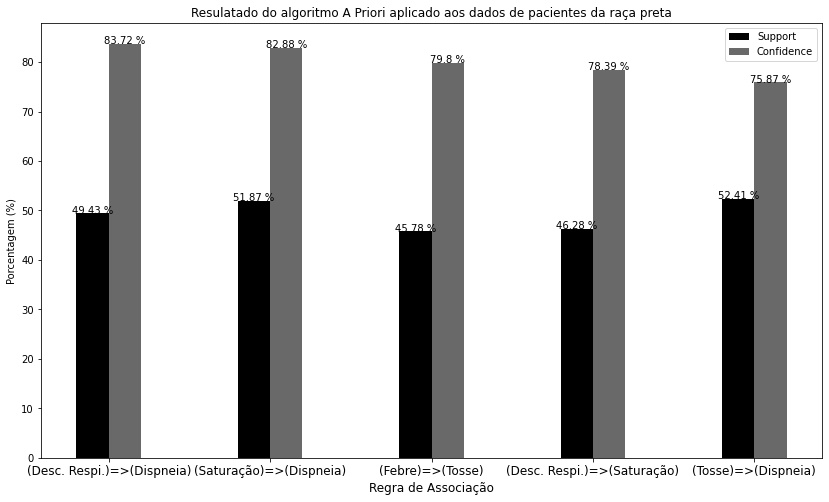
\includegraphics[width=14cm]{1_Preta_apriori.jpg}
    \caption{Resultado gráfico do A Priori relacionando sintomas dos pacientes da raça preta}
    \end{figure}
    
    \begin{itemize}
    \item 49,43\% dos pacientes da raça preta que tiveram desconforto respiratório manifestaram também dispneia, sendo a confiança dessa regra acorrer de 83,72\%;
    
    \item 51,87\% dos pacientes da raça preta que tiveram saturação manifestaram também dispneia, sendo a confiança dessa regra acorrer de 82,88\%;
    
    \item 45,78\% dos pacientes da raça preta que tiveram febre manifestaram tosse, sendo a confiança dessa regra acorrer de 79,8\%;
    
    \item 46,28\% dos pacientes da raça preta que tiveram desconforto respiratório manifestaram saturação, sendo a confiança dessa regra acorrer de 78,39\%;
    
    \item 52,41\% dos pacientes da raça preta que tiveram tosse manifestaram também dispneia, sendo a confiança dessa regra acorrer de 75,87\%;
    \end{itemize}
    
    Entre pacientes pretos a associação de sintomas que mais ocorre entre os casos é a de que se tiver a pessoa tiver saturação terá consequentemente dispneia, essa regra ocorre em cerca de 51,87\% dos casos. Conferindo a confiança podemos afirmar que a maior probabilidade de uma regra ser verdadeira e a que se a pessoa preta tiver desconforto respiratório terá dispneia.
    
    \begin{figure}[!h]
    \centering
    
\includegraphics[width=3.3cm]{fund0.png}
    \end{figure}
    
    \begin{figure}[!h]
    \centering
    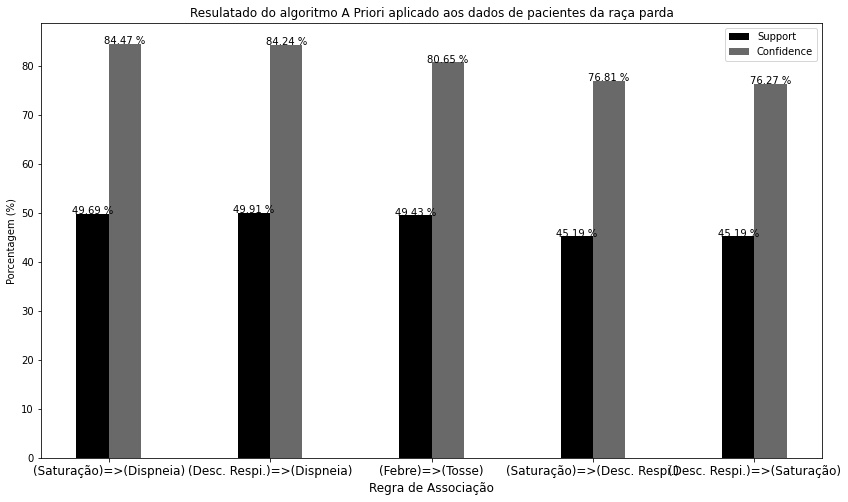
\includegraphics[width=14cm]{1_Parda_apriori.jpg}
    \caption{Resultado gráfico do A Priori relacionando sintomas dos pacientes da raça parda}
    \end{figure}
    
  \begin{itemize}
    \item 49,69\% dos pacientes da raça parda que tiveram saturação manifestaram também dispneia, sendo a confiança dessa regra acorrer de 84,47\%;
    
    \item 49,81\% dos pacientes da raça parda que tiveram desconforto respiratória manifestaram também dispneia, sendo a confiança dessa regra acorrer de 84,24\%;
    
    \item 49,43\% dos pacientes da raça parda que tiveram febre manifestaram tosse, sendo a confiança dessa regra acorrer de 80,65\%;
    
    \item 45,19\% dos pacientes da raça parda que tiveram saturação manifestaram desconforto respiratório, sendo a confiança dessa regra acorrer de 76,81\%;
    
    \item 45,19\% dos pacientes da raça preta que tiveram desconforto respiratório manifestaram também saturação, sendo a confiança dessa regra acorrer de 76,27\%;
    \end{itemize}
    
    Nos pacientes pardos a associação de sintomas que mais ocorre entre os casos a que se a pessoa tiver desconforto respiratório terá dispneia, essa regra ocorre em cerca de 49,91\% dos casos. Observando a confiança podemos afirmar que a maior probabilidade de uma regra ser verdadeira entre os pardos e é a de que se a pessoa tiver saturação terá consequentemente dispneia.
    
    \begin{figure}[!h]
    \centering
    
\includegraphics[width=3.3cm]{fund0.png}
    \end{figure}
    
    \begin{figure}[!h]
    \centering
    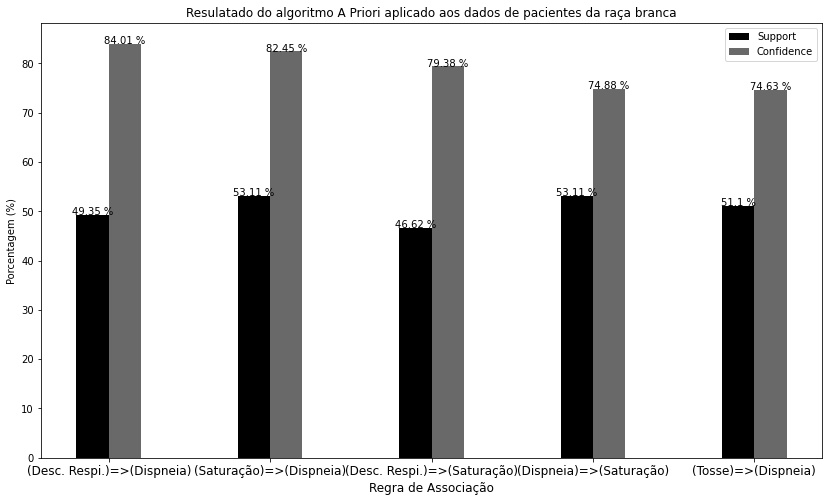
\includegraphics[width=14cm]{1_Branca_apriori.jpg}
    \caption{Resultado gráfico do A Priori relacionando sintomas dos pacientes da raça branca}
    \end{figure}
    
    \begin{itemize}
    
    \item 49,35\% dos pacientes da raça branca que tiveram desconforto respiratória manifestaram também dispneia, sendo a confiança dessa regra acorrer de 84,01\%;
    
    \item 53,11\% dos pacientes da raça branca que tiveram saturação manifestaram também dispneia, sendo a confiança dessa regra acorrer de 82,45\%;
    
    \item 46,62\% dos pacientes da raça branca que tiveram desconforto respiratória manifestaram saturação, sendo a confiança dessa regra acorrer de 79,38\%;
    
    \item 53,11\% dos pacientes da raça branca que tiveram dispneia manifestaram saturação, sendo a confiança dessa regra acorrer de 74,88\%;
    
    \item 51,1\% dos pacientes da raça branca que tiveram tosse manifestaram também dispneia, sendo a confiança dessa regra acorrer de 74,63\%;
    \end{itemize}
    
    Temos que entre os pacientes brancos a associação de sintomas que mais ocorre entre os casos a que se a pessoa tiver dispneia terá saturação, sendo essa afirmação valida também para a associação ao contrario (saturação resultando dispneia).Logo com a confiança pode-se afirmar que a associação desconforto respiratório implica dispneia tem a maior probabilidade de ser uma regra verdadeira entre os brancos.
    
    Sabe-se que o maior índice de casos ocorre entre pessoas brancas seguido de pessoas pardas, sendo que pessoas pretas tem um dos menores índices de ocorrência. Logo sobre a relação dos dados raciais e de sintomas em comum, vemos que em pardos e brancos saturação implicando dispneia é a associação os que mais ocorre, já em pretos tosse implicando dispneia é tem maior ocorrência. 
    
    Considerando a confiança concluímos que nos pacientes pretos e brancos a associação desconforto respiratório implica dispneia tem a maior probabilidade de ser uma regra verdadeira entre esses dados, e que em pardos é a associação saturação resultando ter dispneia a maior.
    
    \begin{figure}[!h]
    \centering
    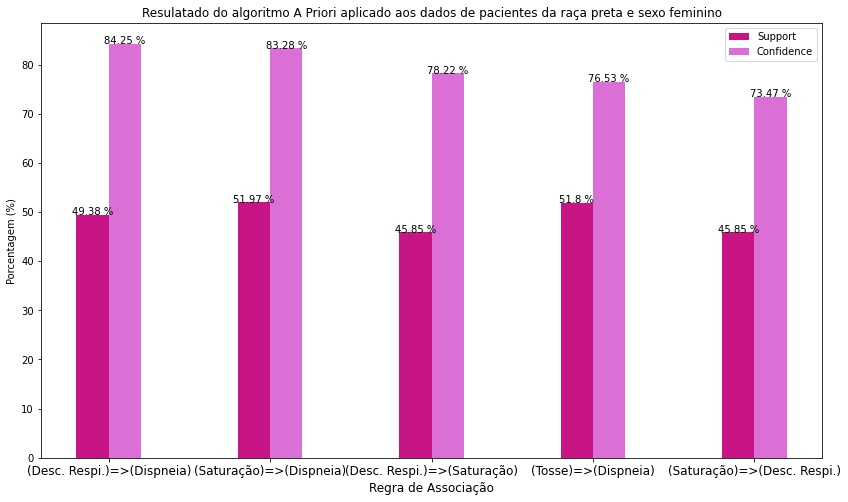
\includegraphics[width=7.5cm]{1_Preta_feminino_apriori.jpg}
    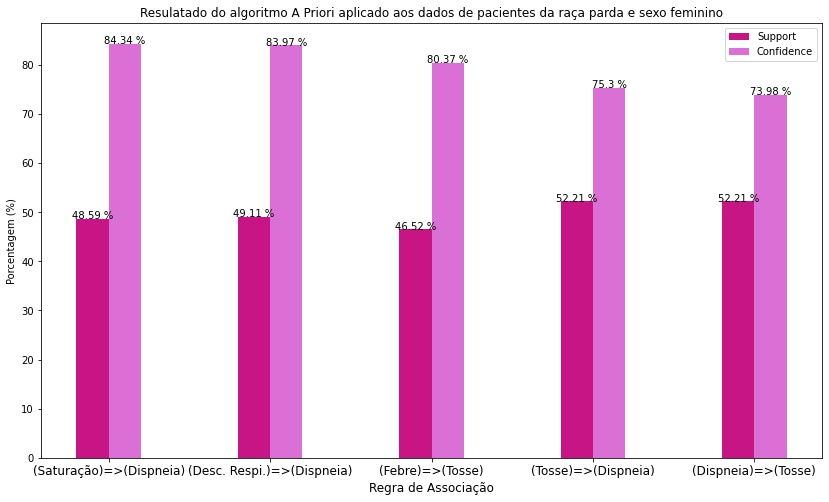
\includegraphics[width=7.5cm]{1_Parda_feminina_apriori.jpg}
    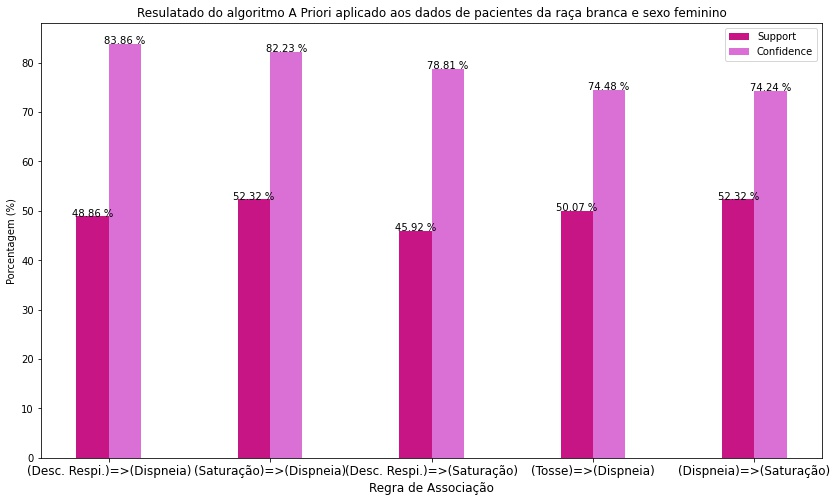
\includegraphics[width=8cm]{1_Branca_feminino_apriori.jpg}
    \caption{Gráficos dos resultados do relacionamento do sexo feminino e raça dos pacientes de covid-19}
    \end{figure}
    
    O primeiro gráfico trás os pacientes do sexo feminino e da raça preta e suas associações de sintomas, vemos que a que mais aparece entre as regras de associação e a que saturação implica ter dispneia, com 51,97\% entre os casos. Medindo a confiança, temos que desconforto respiratório resultando em ter dispneia como a regra com a maior probabilidade de ser verdadeira, com o valor de 84,25\%.
    
    No segundo mostra os pacientes do sexo feminino e da raça parda e suas regras de associações de sintomas, onde temos que o maior incidente é a regra tosse resultando dispneia e o contrario também, dispneia resultando tosse, ambos com 52,21\%. Com a confiança temos que saturação provocando dispneia no paciente como a associação com maior probabilidade de ser verdadeira.
    
     Agora no terceiro e ultimo gráfico exibe-se os dados dos pacientes do sexo feminino e raça branca e as regras de associação de sintomas que essas características tem dentro da base, vemos que a regra dispneia resultando a pessoas ter saturação junto como o inverso (saturação implicando dispneia) como as como maior ocorrência entre os pacientes com essas características, sendo de 52,32\% . A confiança declara que desconforto respiratório provocando a pessoa com covid-19 ter dispneia é a associação com maior valor de ser verdadeira, 83,86\%.
     
    
    \begin{figure}[!h]
    \centering
    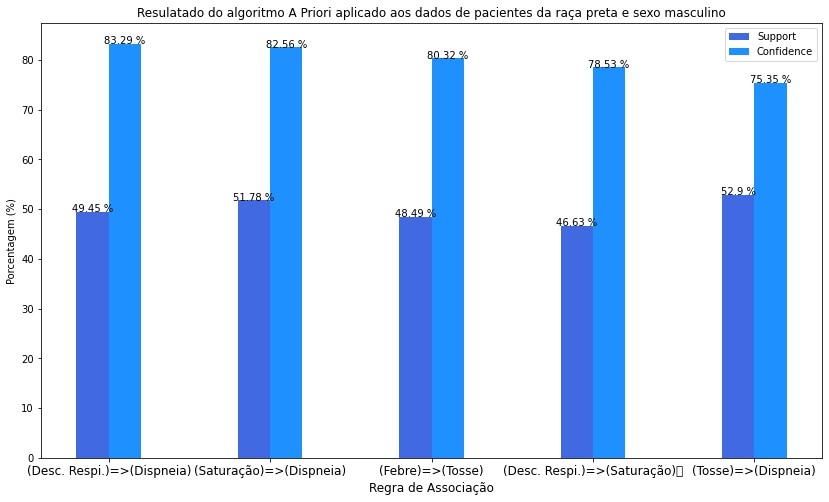
\includegraphics[width=7.5cm]{1_Preta_masculino_apriori.jpg}
    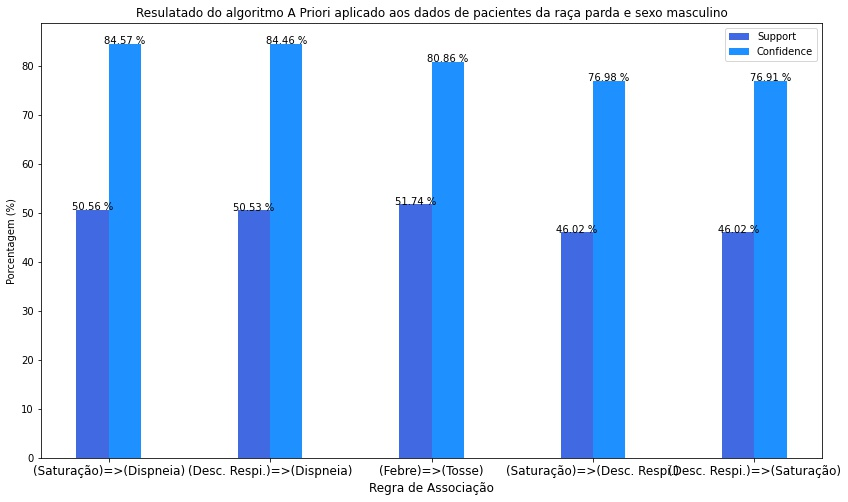
\includegraphics[width=7.5cm]{1_Parda_masculino_apriori.jpg}
    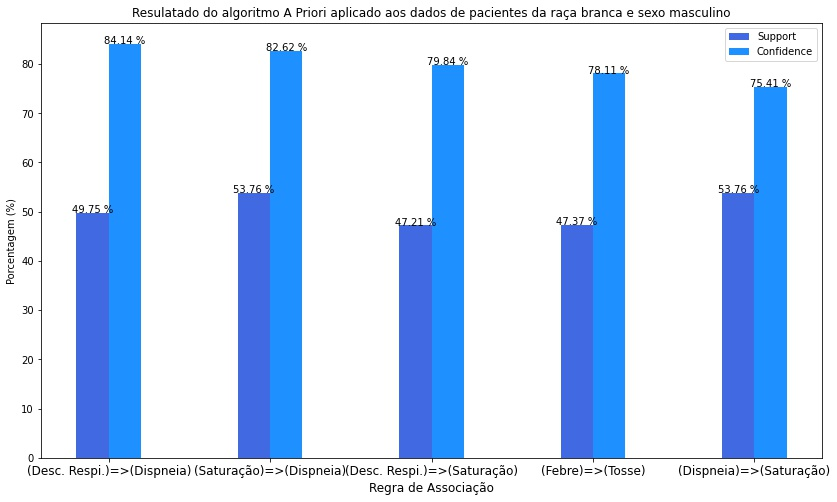
\includegraphics[width=7.5cm]{1_Branca_masculino_apriori.jpg}
    \caption{Gráficos dos resultados do relacionamento do sexo masculino e a raça dos pacientes}
    \end{figure}
    
    Na figura 31 temos no primeiro gráfico os dados de pacientes do sexo masculino e raça preta e suas regras de associação de sintomas, temos como a maior ocorrência a regra tosse implicando dispneia, sendo 52\% de vezes que apareceu entre esses dados. Como maior confiança de ser uma regra verdadeira temos desconforto respiratório implicando dispneia, com 83,29\%.
    
    Segundo gráfico é dos pacientes do sexo masculino e raça parda com as regras de associação entre esse perfil, vemos que a regra com maior valor de incidência é febre resultando a pessoa ter tosse, como o numero de 51,74\%. A confiança de ser uma regra verdadeira com maior valor temos saturação resultando a pessoa ter dispneia, com 84\%.
    
    No ultimo gráfico da figura 31 mostra-se, os pacientes do sexo masculino e raça branca e suas regras de associação de sintomas, a regra de maior ocorrência é saturação implicando o paciente ter dispneia, e vise e versa, como o valor de 53,76\%. Como regra de maior confiança de ser verdadeira temos desconforto respiratório provocando o paciente ter dispneia também, com valor de 84,14\%.
    
    
    
    Para finalizar o projeto, pode-se dizer que conseguimos chegar em alguns conhecimentos interessantes a cerca dos dados. Um ponto importante observado é que os resultados foram afetados porque alguns sintomas são muito semelhantes, assim podendo causar certa monotonia entre os resultados dificultando uma melhora visão do que se tem em cada ponto trabalhado.

\chapter{Cronograma de atividades}
A descrição das atividades remanescentes está listada na Tabela \ref{tb:atividades}, enquanto que o cronograma é apresentado na Tabela \ref{tb:cronograma}.

%%%% INICIO ATIVIDADES PREVISTAS %%%%%%%%%%%%%%%%%

\setstretch{1} 
\begin{table}[!h]
  \centering
  \caption{Lista de atividades previstas.}\label{tb:atividades}
  \begin{tabular}{cp{9.4cm}}
    \hline \hline &\\[-0.4cm]
    {\bf Atividades} & \multicolumn{1}{c}{\bf Descrição} \\
    \hline
    &\\[-0.4cm]
    \textbf{A} & Obtenção dos dados.\\[0.2cm]
    \textbf{B} & Fazer a Analise estatística dos dados e limpar a base.\\[0.2cm]
    \textbf{C} & Descrição dos dados.\\[0.2cm]
    \textbf{D} & Escolher e utilizar o algoritmo de Mineração de Dados.\\[0.2cm]
    \textbf{E} & Obtenção de resultados\\[0.2cm]
    \textbf{F} &  Avaliação dos resultados e descoberta de conhecimento\\[0.2cm]
    \textbf{G} &  Escrita da Monografia\\[0.2cm]
    \hline \hline
  \end{tabular}
\end{table}

%%% FIM ATIVIDADES PREVISTAS %%%%%%%%%%%%%%%%%


%%%%% INICIO DO CRONOGRAMA %%%%%%%%%%%%%%

\begin{table}[!h]
  \centering \fontsize{8}{12}%\tiny
  \caption{Cronograma de Atividades}\label{tb:cronograma}
  \begin{tabular}{|c|c|c|c|c|c|c|c|c|c|c|}
    \hline
    {\normalsize\bf Ano}  &\multicolumn{9}{c|}{\normalsize\bf 2021/2022}\\
    \hline
 {\normalsize\bf Mês} &
 \multirow{2}*{\bf Out}&\multirow{2}*{\bf Nov}&\multirow{2}*{\bf Dez}& \multirow{2}*{\bf Jan}&\multirow{2}*{\bf Fev}&\multirow{2}*{\bf Mar}&\multirow{2}*{\bf Abr}&\multirow{2}*{\bf Mai}&\multirow{2}*{\bf Jun}\\
   \cline{1-1}
{\bf Atv.}    & & & & & & & & &    \\
\hline
{\normalsize\bf A} &$\surd$ & & & & & & & &  \\
\hline
{\normalsize\bf B} & $\surd$ & & & & & & & &\\
\hline
%\hhline{>{\arrayrulecolor{black}}---->{\arrayrulecolor{black}}->{\arrayrulecolor{black}}------}
{\normalsize\bf C} & &$\surd$ & & & & & & & \\
\hline
%\hhline{>{\arrayrulecolor{black}}----->{\arrayrulecolor{black}}-->{\arrayrulecolor{black}}----}
{\normalsize\bf D}& & & $\surd$ &$\surd$ & & & & &  \\
%\hhline{>{\arrayrulecolor{black}}------>{\arrayrulecolor{black}}->{\arrayrulecolor{black}}----}
\hline
{\normalsize\bf E}& & & & & $\surd$ &$\surd$ & & &    \\
%\hhline{>{\arrayrulecolor{black}}------->{\arrayrulecolor{black}}->{\arrayrulecolor{black}}---}
\hline
{\normalsize\bf F} & & & & & & &$\surd$ & &   \\
% \hhline{>{\arrayrulecolor{black}}-------->{\arrayrulecolor{black}}-->{\arrayrulecolor{black}}-}
\hline
{\normalsize\bf G}& & & & & & & &$\surd$ &$\surd$   \\
% \hhline{>{\arrayrulecolor{black}}-------->{\arrayrulecolor{black}}-->{\arrayrulecolor{black}}-}
\hline
  \end{tabular}
\end{table}


\backmatter 
\singlespacing   
% ----------------------------------------------------------------------------------------------------- %
\bibliography{tcc_exemplo}
\end{document}
